\documentclass[a4paper,12pt]{report}
\usepackage{fontspec} % Handles fonts in XeLaTeX. Replaces inputenc and fontenc.
\usepackage{geometry}
\geometry{margin=1in}
\usepackage{graphicx}
\usepackage[colorlinks=true, linkcolor=blue, citecolor=blue]{hyperref} % Made links active
\usepackage{titlesec}
\usepackage{setspace}
\usepackage{wrapfig}
\usepackage{subcaption} % Modern replacement for 'subfigure'
\usepackage{listings}
\usepackage{xcolor}
\usepackage{csquotes}
\usepackage{ragged2e}
\usepackage{lipsum}
\usepackage{pdfpages}
\usepackage{amsmath}
\usepackage{amssymb} % For math symbols
\usepackage[acronym]{glossaries} % For automatic abbreviations
\usepackage{tocloft}
\usepackage{cite}
\usepackage{float}
\usepackage{bibentry}
\usepackage{xcolor}
\usepackage{multirow}
\usepackage{siunitx}
\usepackage{enumitem}
\usepackage{fancyhdr}
\usepackage{comment}
\usepackage{tabularx}
\usepackage{booktabs}
\usepackage{makecell}% provides \makecell
\usepackage{array}% for >{\raggedright\arraybackslash}X

% --- ADDED: Acronym Definitions ---
% Since I don't have your 'glossary.tex' file, I have defined the
% acronyms found in your document here.
\newacronym{cnn}{CNN}{Convolutional Neural Network}
\newacronym{lstm}{LSTM}{Long Short-Term Memory}
\newacronym{stalta}{STA/LTA}{Short-Term Average/Long-Term Average}
\newacronym{mfcc}{MFCC}{Mel-Frequency Cepstral Coefficient}
\newacronym{eew}{EEW}{Earthquake Early Warning}
\newacronym{ml}{ML}{Machine Learning}
\newacronym{dl}{DL}{Deep Learning}
\newacronym{snr}{SNR}{Signal-to-Noise Ratio}
\newacronym{fft}{FFT}{Fast Fourier Transform}
\newacronym{stft}{STFT}{Short-Time Fourier Transform}
\newacronym{dct}{DCT}{Discrete Cosine Transform}
\newacronym{pesmos}{PESMOS}{Program for Excellence in Strong Motion Studies}
\newacronym{egmb}{EGMB}{Eastern Ghats Mobile Belt}
\newacronym{awg}{AWG}{Arbitrary Waveform Generator}
% --- End of Acronyms ---


% Create the glossary
\makeglossaries

% --- Customizations for ToC, LoF, LoT (Remove dot leaders) ---
\renewcommand{\cftchapleader}{\hfil} % Removes dots for chapters in ToC
\renewcommand{\cftsecleader}{\hfil}% Removes dots for sections in ToC
\renewcommand{\cftsubsecleader}{\hfil}% Removes dots for subsections in ToC
\renewcommand{\cftfigleader}{\hfil}% Removes dots for figures in LoF
\renewcommand{\cfttableader}{\hfil}% Removes dots for tables in LoT

% Keep your existing ToC/LoF customizations
\renewcommand{\cfttoctitlefont}{\centering\Huge\bfseries\color{blue}}
\renewcommand{\cftsecfont}{\normalfont}
\renewcommand{\cftsubsecfont}{\normalfont}
\renewcommand{\cftsubsubsecfont}{\normalfont}
\setlength{\cftbeforetoctitleskip}{0pt}
\setlength{\cftbeforesubsecskip}{0pt}

% For the list of figures
\renewcommand{\listfigurename}{List of Figures}
\renewcommand{\cftloftitlefont}{\centering\Large\bfseries\color{blue}}

% For the list of tables (add this if you haven't already)
\renewcommand{\listtablename}{List of Tables}
\renewcommand{\cftlottitlefont}{\centering\Large\bfseries\color{blue}}
% --- End Customizations ---

% --- NEW: Replicating your manual chapter/section style ---
% This makes \chapter{} look like your manual formatting
\titleformat{\chapter}[display]
{\normalfont\Large\bfseries\centering} % Format for the whole block
{\chaptertitlename\ \thechapter} % "CHAPTER X"
{0.2cm} % Space between "CHAPTER X" and title
{\Large\textbf} % Format for the title text
\titlespacing*{\chapter}{0pt}{0pt}{0.5cm} % left, before, after

% This makes \section{} look like your manual formatting
\titleformat{\section}
{\normalfont\fontsize{14pt}{12pt}\selectfont\bfseries} % Format
{\thesection} % Number (e.g., "4.1")
{1em} % Space after number
{} % Code before title

% This makes \subsection{} look like your manual formatting
\titleformat{\subsection}
{\normalfont\fontsize{13pt}{12pt}\selectfont\bfseries} % Format
{\thesubsection} % Number (e.g., "2.1.1")
{1em} % Space after number
{} % Code before title
% --- END OF NEW FORMATTING ---

% --- ADDED: Remove paragraph indentation globally ---
\setlength{\parindent}{0pt}
% ---

\begin{document}
\begin{center}
    \Large\textbf{{\textbf{SEISMIC DETECTION, VISUALIZATION\\ AND ANALYSIS
}}}
\end{center}
\vspace{.1cm}


\begin{center}
        {\large {A MAIN PROJECT REPORT} \\[0.5cm]
    Submitted by \\[0.3cm]
    \large \textbf{NISSA ANN SAJI(MBC22CS053)} \\[0.3cm]
    \large \textbf{JUSTINE BIJU PAUL(MBC22CS044)} \\[0.3cm]
    \large \textbf{ALLAN SHIBU KOSHY(MBC22CS016)} \\[0.3cm]
    \large \textbf{BIJIN BINOY MATHEW(MBC22CS026)} \\[0.3cm]
    to\\[0.3cm]
    {APJ Abdul Kalam Technological University} \\
    { In partial fulfillment of requirements for the award of degree} \\[0.5cm]
    of\\[0.3cm]
    {\Large \textbf{Bachelor of Technology}} \\[0.3cm]
    {in} \\[0.5cm]
    {\Large \textbf{Computer Science and Engineering}} \\[0.5cm]
    }
    
\end{center}


\vspace{0.5cm}
\begin{figure}[h]
    \centering
    
\includegraphics[width=0.3\textwidth]{MBC.jpg}
\end{figure}
\vspace{1.3cm}

\begin{center}
\noindent\mbox{{\textbf{DEPARTMENT OF COMPUTER SCIENCE AND ENGINEERING}}} \\[0.1cm]
{\textbf{\small{MAR BASELIOS CHRISTIAN COLLEGE OF ENGINEERING AND TECHNOLOGY, PEERMADE}}} \\[0.5cm]
{\textbf{MARCH 2026}}
\end{center}

\thispagestyle{empty}
\begin{center}
    \Large\textbf{{\textbf{SEISMIC DETECTION, VISUALIZATION\\ AND ANALYSIS
}}}
\end{center}
\vspace{.1cm}


\begin{center}
        {\large {A MAIN PROJECT REPORT} \\[0.5cm]
    Submitted by \\[0.3cm]
    \large \textbf{NISSA ANN SAJI(MBC22CS053)} \\[0.3cm]
    \large \textbf{JUSTINE BIJU PAUL(MBC22CS044)} \\[0.3cm]
    \large \textbf{ALLAN SHIBU KOSHY(MBC22CS016)} \\[0.3cm]
    \large \textbf{BIJIN BINOY MATHEW(MBC22CS026)} \\[0.3cm]
    to\\[0.3cm]
    {APJ Abdul Kalam Technological University} \\
    { In partial fulfillment of requirements for the award of degree} \\[0.5cm]
    of\\[0.3cm]
    {\Large \textbf{Bachelor of Technology}} \\[0.3cm]
    {in} \\[0.5cm]
    {\Large \textbf{Computer Science and Engineering}} \\[0.5cm]
    }
    
\end{center}


\vspace{0.5cm}
\begin{figure}[h]
    \centering
    
\includegraphics[width=0.3\textwidth]{MBC.jpg}
\end{figure}
\vspace{1.3cm}

\begin{center}
\noindent\mbox{{\textbf{DEPARTMENT OF COMPUTER SCIENCE AND ENGINEERING}}} \\[0.1cm]
{\textbf{\small{MAR BASELIOS CHRISTIAN COLLEGE OF ENGINEERING AND TECHNOLOGY, PEERMADE}}} \\[0.5cm]
{\textbf{MARCH 2026}}
\end{center}

\thispagestyle{empty}
\vspace{2cm}
\begin{center}
\noindent \mbox{{\textbf{DEPARTMENT OF COMPUTER SCIENCE AND ENGINEERING}}} \\[0.4cm]
\textbf {\small MAR BASELIOS CHRISTIAN COLLEGE OF ENGINEERING AND TECHNOLOGY} \\[0.4cm]
\textbf{2025-2026}
\end{center}
\vspace{0.5cm}
\begin{figure}[h]
    \centering
    
\includegraphics[width=0.3\textwidth]{MBC.jpg}
\end{figure}

\begin{center}
    \Large\textbf{CERTIFICATE}
\end{center}

%\addcontentsline{toc}{chapter}{\numberline{}Abstract}%
\vspace{1cm}

\fontsize{12pt}{18pt}\selectfont

This is to certify that this report entitled \textbf{\enquote {SEISMIC DETECTION, VISUALIZATION AND ANALYSIS}}  submitted by \textbf{ALLAN SHIBU KOSHY(MBC22CS016)}, \textbf{BIJIN BINOY MATHEW(MBC22CS026)}, \textbf{JUSTINE BIJU PAUL (MBC22-\\CS044)} and \textbf{NISSA ANN SAJI(MBC22CS053)} to the APJ Abdul Kalam Technological University in fulfillment of the requirements for the award of the degree of B.Tech. in Computer Science and Engineering, is a bonafide report of the main project carried out by them under our guidance and supervision. This report in any form has not been submitted to any other University or Institute for any purpose. 
\par

\vspace{2cm} % Space before signatures

% Use minipages to create two blocks and \hfill to push them apart
\noindent % Prevent indentation
\begin{minipage}[t]{0.45\textwidth} % Left block (adjust width as needed)
    \centering % Center text *within* this block
    \textcolor{red}{\textbf{Prof. Josmy George}} \\
    Project Guide \\
    Associate Professor \\
    Department of CSE
\end{minipage}% % No space between minipages
\hfill % Pushes the blocks to opposite sides
\begin{minipage}[t]{0.45\textwidth} % Right block (adjust width as needed)
    \centering % Center text *within* this block
    \textcolor{red}{\textbf{Dr. Ushus Maria Joseph}} \\
    Head of the Department \\
    Associate Professor \\
    Department of CSE
\end{minipage}

\thispagestyle{empty}



\thispagestyle{empty}

% --- CORRECTED FRONT MATTER ---
\pagenumbering{roman} % Start roman numerals
\vspace{2cm}

% --- Abstract and Acknowledgement are correct ---
\chapter*{DECLARATION}
\addcontentsline{toc}{chapter}{\textit{Declaration}} % This adds it to the ToC
\vspace{1cm}

\fontsize{12pt}{18pt}\selectfont
We hereby declare that this report entitled \textbf{\enquote {SEISMIC DETECTION, VISUALIZATION AND ANALYSIS}} is a bonafide record of the preliminary project work carried out by us under the supervision of \textbf{Prof. Josmy George} in the Department of Computer Science and Engineering, Mar Baselios Christian College of Engineering and Technology, Peermade. The project proposal presented in this report has not been presented for the award of any other degrees.\\
\\
Peermade \\
\\
Date: 25 October 2025 \\
\\
\\
\\
\\
\begin{spacing}{1}
	
	\begin{table}[h!]
		\centering
		\begin{tabular}{p{0.5cm} p{6cm} p{10cm}}
\textbf{} && \textbf{ALLAN SHIBU KOSHY(MBC22CS016)} \\[0.3cm]
\textbf{} && \textbf{BIJIN BINOY MATHEW(MBC22CS026)} \\[0.3cm]
\textbf{} && \textbf{JUSTINE BIJU PAUL(MBC22CS044)} \\[0.3cm]
			\textbf{} && \textbf{NISSA ANN SAJI(MBC22CS053)} \\[0.3cm]
		\end{tabular}
	\end{table}
\end{spacing}
\newpage

\newpage
\begin{center}
    \textbf{\underline{COLLEGE VISION \& MISSION}}
\end{center}
\vspace{0.5cm}

\noindent \textbf{VISION} \\[0.2cm]
An Engineering Institute with global quality to groom competent engineers equipped to address the changing needs of society.
\vspace{0.5cm}

\noindent \textbf{MISSION} \\[0.2cm]
Our efforts are dedicated for developing a learner centric education environment to:
\begin{enumerate}
    \item Provide value-based technical learning
    \item Practice real world problem solving
    \item Foster team work in engineering design
    \item Inspire innovations and R\&D
\end{enumerate}
\vspace{1cm}

\begin{center}
    \textbf{\underline{DEPARTMENT VISION \& MISSION}}
\end{center}
\vspace{0.5cm}

\noindent \textbf{VISION} \\[0.2cm]
To become an excellent department by empowering the graduates to address the challenges in the fast-changing scenario, adhering to ethical values.
\vspace{0.5cm}

\noindent \textbf{MISSION} \\[0.2cm]
\begin{enumerate}
    \item Inculcate skills to solve complex engineering problems and instill entrepreneurial capabilities.
    \item Equip the students to advance with the recent trends and technology through Research and Innovations in the field of computer science.
    \item Facilitate the development of professional behavior, ethical values and the spirit of service to the society.
\end{enumerate}


% --- PAGE 2 ---
\newpage
% --- PROGRAMME EDUCATIONAL OBJECTIVES ---
\begin{center}
    \textbf{\underline{PROGRAMME EDUCATIONAL OBJECTIVES (PEOs)}}
\end{center}
\vspace{0.5cm}

\noindent \textbf{Our Graduates will be able to:}
\begin{itemize}[leftmargin=2.5cm]
    \item[\textbf{PEO1:}] Think creatively and critically to solve problems in a global context with varying complexity.
    \item[\textbf{PEO2:}] Exhibit leadership qualities, Ethical Values, managerial and entrepreneurship skills.
    \item[\textbf{PEO3:}] Contribute inventions and innovative advancements in information technology through life-long learning in a sustainable manner.
\end{itemize}

\vspace{1cm}

% --- PROGRAM OUTCOMES ---
\begin{center}
    \textbf{\underline{PROGRAM OUTCOMES (POs)}}
\end{center}
\vspace{0.5cm}

\noindent \textbf{Engineering Graduates will be able to:}
\begin{itemize}[leftmargin=2.5cm]
    \item[\textbf{PO1.}] \textbf{Engineering Knowledge:} Apply the knowledge of mathematics, science, engineering fundamentals, and an engineering specialization to the solution of complex engineering problems.
    
    \item[\textbf{PO2.}] \textbf{Problem Analysis:} Identify, formulate, review research literature, and analyse complex engineering problems reaching substantiated conclusions using first principles of mathematics, natural sciences, and engineering sciences.
    
    \item[\textbf{PO3.}] \textbf{Design/Development of Solutions:} Design solutions for complex engineering problems and design system components or processes that meet the specified needs with appropriate consideration for the public health and safety, and the cultural, societal, and environmental considerations.
    
    \item[\textbf{PO4.}] \textbf{Conduct Investigations of Complex Problems:} Use research-based knowledge and research methods including design of experiments, analysis and interpretation of data, and synthesis of the information to provide valid conclusions.
    
    \item[\textbf{PO5.}] \textbf{Modern Tool Usage:} Create, select, and apply appropriate techniques, resources, and modern engineering and IT tools including prediction and modelling to complex engineering activities with an understanding of the limitations.
    
    \item[\textbf{PO6.}] \textbf{The Engineer and Society:} Apply reasoning informed by the contextual knowledge to assess societal, health, safety, legal and cultural issues and the consequent responsibilities relevant to the professional engineering practice.
    
    \item[\textbf{PO7.}] \textbf{Environment and Sustainability:} Understand the impact of the professional engineering solutions in societal and environmental contexts, and demonstrate the knowledge of, and need for sustainable development.
    
    \item[\textbf{PO8.}] \textbf{Ethics:} Apply ethical principles and commit to professional ethics and responsibilities and norms of the engineering practice.
    
    \item[\textbf{PO9.}] \textbf{Individual and Team Work:} Function effectively as an individual, and as a member or leader in diverse teams, and in multidisciplinary settings.
    
    \item[\textbf{PO10.}] \textbf{Communication:} Communicate effectively on complex engineering activities with the engineering community and with society at large, such as, being able to comprehend and write effective reports and design documentation, make effective presentations, and give and receive clear instructions.
    
    \item[\textbf{PO11.}] \textbf{Project Management and Finance:} Demonstrate knowledge and understanding of the engineering and management principles and apply these to one's own work, as a member and leader in a team, to manage projects and in multidisciplinary environments.
    
    \item[\textbf{PO12.}] \textbf{Life-long learning:} Recognize the need for, and have the preparation and ability to engage in independent and life-long learning in the broadest context of technological change.
\end{itemize}

\vspace{1cm}

% --- PROGRAM SPECIFIC OUTCOMES ---
\begin{center}
    \textbf{\underline{PROGRAM SPECIFIC OUTCOMES (PSOs)}}
\end{center}
\vspace{0.5cm}

\begin{itemize}[leftmargin=2.5cm]
    \item[\textbf{PSO1:}] Apply theoretical and practical knowledge to analyse and model hardware systems with varying complexity.
    \item[\textbf{PSO2:}] Utilize modern programming platforms, tools and logical reasoning skills to analyse and develop application software.
    \item[\textbf{PSO3:}] Apply computational and networking skills to solve and develop secure communication environment.
\end{itemize}

% --- PAGE 4 ---
\newpage
\subsection*{COURSE OUTCOMES (COs)}

\vspace{0.3cm}
\noindent \textbf{Course Outcomes [COs]:} After successful completion of the course, the students will be able to:

\vspace{0.3cm}
\noindent
\begin{tabularx}{\textwidth}{|c|X|}
\hline
CO1 & Model and solve real world problems by applying knowledge across domains (Cognitive knowledge level: \textbf{Apply}). \\ \hline
CO2 & Develop products, processes or technologies for sustainable and socially relevant applications (Cognitive knowledge level: \textbf{Apply}) \\ \hline
CO3 & Function effectively as an individual and as a leader in diverse teams and to comprehend and execute designated tasks (Cognitive knowledge level: \textbf{Apply}) \\ \hline
CO4 & Plan and execute tasks utilizing available resources within timelines, following ethical and professional norms (Cognitive knowledge level: \textbf{Apply}) \\ \hline
CO5 & Identify technology/research gaps and propose innovative/creative solutions (Cognitive knowledge level: \textbf{Analyze}) \\ \hline
CO6 & Organize and communicate technical and scientific findings effectively in written and oral forms (Cognitive knowledge level: \textbf{Apply}) \\ \hline
\end{tabularx}

\vspace{1cm}
\noindent
\begin{tabularx}{\textwidth}{|c|*{12}{>{\centering\arraybackslash}X|}}
\hline
 & PO1 & PO2 & PO3 & PO4 & PO5 & PO6 & PO7 & PO8 & PO9 & PO10 & PO11 & PO12 \\ \hline
CO1 & 2 & 2 & 2 & 1 & 2 & 2 & 2 & 1 & 1 & 1 & 1 & 2 \\ \hline
CO2 & 2 & 2 & 2 & & 1 & 3 & 3 & 1 & 1 & & 1 & 1 \\ \hline
CO3 & & & & & & & & & 3 & 2 & 2 & 1 \\ \hline
CO4 & & & & 2 & & & 3 & 2 & 2 & 3 & 2 & \\ \hline
CO5 & 2 & 3 & 3 & 1 & 2 & & & & & & & 1 \\ \hline
CO6 & & & & & 2 & & & 2 & 2 & 3 & 1 & 1 \\ \hline
\end{tabularx}
\newpage
%------------------SDG INTEGRATION------------------

\begin{center}
    \textbf{\large SUSTAINABLE DEVELOPMENT GOALS (SDGS) INTEGRATION} 
\end{center}

The Sustainable Development Goals (SDGs) are a set of 17 global goals established by the United Nations to address major global challenges such as health, safety, equality, innovation, and social well-being. Integrating SDGs into our project ensures that the system contributes not only technologically but also socially by promoting safer digital communication and protecting individuals from psychological harm.

\subsection*{SDGs Integrated in Our Project}
\begin{itemize}[leftmargin=2.5cm]
    \item[\textbf{SDG 3:}] \textbf{Good Health and Well-being} -- The system identifies psychological manipulation and abusive communication that can impact mental health. Early detection supports emotional well-being and promotes healthier interactions.
    \item[\textbf{SDG 9:}] \textbf{Industry, Innovation, and Infrastructure} -- The project uses advanced technologies such as transformer-based models, real-time analysis, and modern web frameworks to build an innovative and scalable digital safety solution.
    \item[\textbf{SDG 16:}] \textbf{Peace, Justice, and Strong Institutions} -- By detecting manipulation and harmful communication, the system helps reduce online abuse and promotes safer digital environments. It also supports documentation for professional or legal use.
    \item[\textbf{SDG 4:}] \textbf{Quality Education} -- The system raises awareness of manipulation tactics, helping users recognize harmful communication patterns and improve digital literacy.
\end{itemize}

\begin{table}[h]
\centering
\renewcommand{\arraystretch}{1.3}
\begin{tabular}{|c|c|p{11cm}|}
\hline
\textbf{SDG} & \textbf{Level} & \textbf{Integration} \\
\hline
3 & 5 & Detects psychological manipulation and harmful communication, promoting mental well-being and safer digital interactions \\
\hline
4 & 4 & Improves awareness and understanding of manipulation tactics, enhancing digital literacy and user education \\
\hline
9 & 4 & Utilizes advanced AI, NLP models, and modern web technologies to build an innovative and scalable digital safety system \\
\hline
16 & 5 & Helps reduce online abuse and manipulation, supporting safe, transparent, and accountable digital environments \\
\hline
\end{tabular}
\end{table}
\newpage

\chapter*{ACKNOWLEDGEMENT}
\addcontentsline{toc}{chapter}{\textit{Acknowledgement}} % This adds it to the ToC
\vspace{1cm}

\fontsize{12pt}{18pt}\selectfont


The success of this project was made possible through the guidance and support of many. We 
are grateful to the Management of Mar Baselios Christian College of Engineering and Technology for the opportunity and platform to complete this work. Special thanks to our 
Principal, \textbf{Dr.V I George, Principal}, for his exceptional support and the facilities provided. We deeply appreciate the supervision and assistance we received, which were crucial to the project's completion.  \\
\\
We are extremely indebted to our Head of the Department, \textbf{Dr. Ushus Maria Joseph, Associate Professor} Department of Computer Science and Engineering, for her valuable suggestions and encouragement during the course of our project work. \\
\\
We are grateful to thank our project coordinator, \textbf{Prof. Aryalakshmi R}, Assistant Professor, Department of Computer Science and Engineering for her valuable support. \\
\\
We are deeply grateful to our project guide, \textbf{Prof. Josmy George}, Associate Professor, Department of Computer Science and Engineering, for her keen interest and guidance throughout our project, providing essential information for a successful presentation. We also appreciate the constant encouragement, support, and guidance from all the faculty members of the Department of Computer Science and Engineering, which were instrumental in completing our project work successfully. \\
\vspace{1cm}

\begin{spacing}{1}
	
	\begin{table}[h!]
		\centering
		\begin{tabular}{p{0.5cm} p{6cm} p{10cm}}
\textbf{} && \textbf{ALLAN SHIBU KOSHY(MBC22CS016)} \\[0.3cm]
\textbf{} && \textbf{BIJIN BINOY MATHEW(MBC22CS026)} \\[0.3cm]
\textbf{} && \textbf{JUSTINE BIJU PAUL(MBC22CS044)} \\[0.3cm]
			\textbf{} && \textbf{NISSA ANN SAJI(MBC22CS053)} \\[0.3cm]
		\end{tabular}
	\end{table}
\end{spacing}
\newpage

% --- Abstract and Acknowledgement are correct ---
\chapter*{ABSTRACT}
\addcontentsline{toc}{chapter}{\textit{Abstract}} % This adds it to the ToC
\vspace{1cm}

\fontsize{12pt}{18pt}\selectfont
Earthquake signals are non-stationary in nature and thus in real-time, it is difficult to identify and classify events based on classical approaches like peak ground displacement, peak ground velocity. Even the popular algorithm of STA/LTA requires extensive research to determine basic thresholding parameters so as to trigger an alarm. Also, many times due to human error or other unavoidable natural factors such as thunder strikes or landslides, the algorithm may end up raising a false alarm. This work focuses on detecting earthquakes by converting seismograph recorded data into corresponding audio signals for better perception and then uses popular Speech Recognition techniques of Filter bank coefficients and Mel Frequency Cepstral Coefficients (MFCC) to extract the features. These features
were then used to train a Convolutional Neural Network(CNN) and a Long Short Term Memory
(LSTM) network. The proposed method can overcome the above-mentioned problems and help in
detecting earthquakes automatically from the waveforms without much human intervention. For the 1000Hz audio data set the CNN model showed a testing accuracy of 91.1\% for 0.2-second samplewindow length while the LSTM model showed 93.99\% for the same. A total of 610 sounds consisting of 310 earthquake sounds and 300 non-earthquake sounds were used to train the models. While testing, the total time required for generating the alarm was 1.68 seconds which included individual times for data collection, processing, and prediction. Taking into consideration the processing and prediction delays, the total time is thus considered to be approximately 2 seconds. This shows the effectiveness of the proposed method for EEW applications. Since the input of the method is only the waveform, it is suitable for real-time processing, thus, the models can very well be used also as an onsite earthquake early warning system requiring a minimum amount of preparation time and workload.

\newpage
% --- ToC, LoF, LoT ---
\addcontentsline{toc}{chapter}{\textit{Contents}}
\tableofcontents
\newpage
\addcontentsline{toc}{chapter}{\textit{List of Figures}}
\begingroup
\let\cleardoublepage\clearpage
\listoffigures
% --- Abbreviations ---
\endgroup

\begingroup
\let\clearpage\relax
\let\cleardoublepage\relax
\chapter*{ABBREVIATIONS}
\endgroup
\addcontentsline{toc}{chapter}{\textit{Abbreviations}}
\fontsize{12pt}{18pt}\selectfont
\begin{spacing}{1.5}
\begin{tabular}{p{3.5cm} p{0.5cm} p{10cm}}
\textbf{AI}   & -- & Artificial Intelligence \\
\textbf{AUC}  & -- & Area Under the Curve \\
\textbf{CNN}  & -- & Convolutional Neural Network \\
\textbf{CPU}  & -- & Central Processing Unit \\
\textbf{CSV}  & -- & Comma-Separated Values \\
\textbf{DCT}  & -- & Discrete Cosine Transform \\
\textbf{DL}   & -- & Deep Learning \\
\textbf{EEW}  & -- & Earthquake Early Warning \\
\textbf{FFT}  & -- & Fast Fourier Transform \\
\textbf{GPU}  & -- & Graphics Processing Unit \\
\textbf{GUI}  & -- & Graphical User Interface \\
\textbf{IoT}  & -- & Internet of Things \\
\textbf{JSON} & -- & JavaScript Object Notation \\
\textbf{LSTM} & -- & Long Short-Term Memory \\
\textbf{MAE}  & -- & Mean Absolute Error \\
\textbf{MFCC} & -- & Mel-Frequency Cepstral Coefficient \\
\textbf{ML}   & -- & Machine Learning \\
\textbf{MSE}  & -- & Mean Squared Error \\
\textbf{mseed}& -- & MiniSEED (Standard for Exchange of Earthquake Data) \\
\textbf{OBS}  & -- & Ocean Bottom Seismometer \\
\textbf{P-wave}& -- & Primary Wave \\
\textbf{ReLU} & -- & Rectified Linear Unit \\
\textbf{RNN}  & -- & Recurrent Neural Network \\
\textbf{RMSE} & -- & Root Mean Square Error \\
\textbf{ROC}  & -- & Receiver Operating Characteristic \\
\textbf{S-wave}& -- & Secondary (Shear) Wave \\
\textbf{SNR}  & -- & Signal-to-Noise Ratio \\
\textbf{STA/LTA}& -- & Short-Term Average / Long-Term Average \\
\textbf{STEAD}& -- & Stanford Earthquake Dataset \\
\textbf{STFT} & -- & Short-Time Fourier Transform \\
\end{tabular}
\end{spacing}
\newpage

\pagenumbering{arabic}
\onehalfspacing


\chapter{INTRODUCTION}
\label{chap:introduction}

The field of seismology, particularly in the domain of disaster mitigation, is undergoing rapid transformation driven by the integration of advanced technology, especially deep learning (DL) methods. This introduction outlines the critical importance of Earthquake Early Warning (EEW) systems, details the shift from conventional monitoring techniques to modern deep learning approaches, and explores the diverse and increasingly sophisticated applications of DL in seismic detection, phase picking, event location, and specialized signal classification across various seismic environments.

\section{The Mandate and Constraints of Earthquake Early Warning Systems}
\label{sec:1.1}

Earthquake Early Warning (EEW) systems serve as vital life-saving tools in earthquake-prone regions globally, encompassing countries such as Japan, Taiwan, Mexico, and South Korea. The primary objective of EEW is multifaceted: to provide necessary information to warn the public and inform response actions; to deliver actionable messages leading to safety for populations at risk of imminent threats; and crucially, to minimize response delay.

The urgency inherent in EEW stems from the narrow temporal window available for intervention. Typically, only a matter of seconds separates the initial detection of an earthquake's onset from the arrival of strong, damaging shaking at a target site. While a warning period measured in minutes or hours is generally unachievable, the brief seconds of lead time provided by EEW systems can nonetheless be invaluable for mitigating risk. These seconds enable individuals to take protective actions, such as moving to safer spots within a building or taking proper shelter. Consequently, reducing the lead-time of EEW alerts is a central focus of research. The efficacy of an EEW system relies heavily on the rapidity and reliability of its decision-making process, which is considered more important than the mere transmission of information. Operational considerations also involve managing the alert propagation system, deciding on the system settings for alerts, and ensuring the content of the message is actionable.

The Korea Meteorological Administration (KMA), for instance, operates a network-based EEW service but has recognised the limitations of this traditional technology in achieving sufficiently short warning times and has therefore begun trial testing an on-site warning method.

\section{Evolution of Seismic Signal Detection: From Traditional Methods to Deep Learning}
\label{sec:1.2}

Historically, seismic monitoring systems relied on classical algorithms for detecting the onset of seismic phases. The most widely adopted conventional approach is the Short-Term Average/Long-Term Average (STA/LTA) method, which functions as a power detector. STA/LTA identifies the onset of an earthquake as a sudden change in the ratio between the short-term and long-term amplitude averages of the waveform. While robust, the practical application of STA/LTA in an operational environment, such as an on-site EEW system, demands extensive prerequisites. It requires advance analysis of ambient noise and site-specific structural vibration, along with the tedious process of optimizing threshold values via multiple trials and errors to keep false detections at a minimum. The performance of the STA/LTA algorithm is heavily dependent on having appropriate user-defined thresholds, which must often be customised for different regions.

The exponential growth in seismic data volume, coupled with the rising demand for comprehensive earthquake catalogs, particularly for small or induced events, has necessitated the adoption of automatic detection methods. This need, combined with rapid advancements in Artificial Intelligence (AI), has led to the prominent incorporation of Deep Learning (DL) into seismology.

DL models offer significant advantages over conventional methods. By learning general characteristics of earthquake waveforms from high-level representations, they achieve robust and efficient feature extraction. Importantly, DL networks are capable of automatic feature extraction directly from raw data, eliminating the need for manual feature engineering or specific domain expertise. Furthermore, these networks can exhibit invariance to minor variations in the timing or position of event occurrences. These capabilities allow DL-based seismic phase detection methods to often outperform traditional counterparts.

Key architectural components frequently employed in seismological DL models include:
\begin{itemize}
\item \textbf{Convolutional Neural Networks (CNNs):} CNNs are widely used for earthquake detection and location tasks, capitalizing on their ability to extract relevant features through convolutional layers. CNNs implicitly capture contextual information through multiple levels of abstraction, making them highly effective at detecting local features within multi-dimensional data.
\item \textbf{Recurrent Neural Networks (RNNs) and Long Short-Term Memory (LSTM):} RNNs, particularly those employing Gated Recurrent Units (GRU) or LSTM blocks, are specialized for modeling sequential time-series data. LSTM blocks specifically manage the complexity of long sequences by integrating memory cells and gate mechanisms (input, output, and forget gates), enabling them to capture long-term dependencies in seismic signals.
\item \textbf{Attention Mechanisms and Transformers:} Advanced architectures, such as the Earthquake Transformer (EQT), incorporate attention mechanisms. Attention allows the network to dynamically weight different parts of the seismic sequence based on their relevance to the classification task, focusing on crucial local features while processing the global waveform context.
\end{itemize}

The successful training of these sophisticated models relies on vast, high-quality, labelled datasets. Major initiatives have led to the creation of globally distributed datasets, such as the STanford EArthquake Dataset (STEAD) and the Italian Seismic Data set For Machine Learning (INSTANCE). For instance, STEAD comprises about 1.2 million signals, including both local earthquake waveforms (from various geographic regions) and non-earthquake noise, typically 1-minute long at a 100 Hz sampling rate, recorded at epicentral distances up to 300 km.
\section{Advanced Deep Learning Applications in Seismology}
\label{sec:1.3}

Deep learning models are being deployed to address core seismological tasks with unprecedented efficiency and scope, ranging from microseismic monitoring to real-time earthquake characterization.

\subsection{Phase Picking and Discrimination}
\label{sec:1.3.1}

Reliable phase picking, identifying the arrival times of P- and S-waves, is a fundamental prerequisite for all automatic monitoring pipelines, as it allows for the association of detections with specific events and subsequent location determination.

Leading DL models for phase picking include:
\begin{itemize}
\item \textbf{PhaseNet:} A deep-neural-network-based seismic arrival-time picking method utilizing a U-Net architecture.
\item \textbf{EQTransformer (EQT):} An attentive deep-learning model designed for simultaneous earthquake detection and phase picking. EQT operates as a multi-task network, featuring one deep encoder and three distinct decoders dedicated to predicting the existence of an earthquake signal, P-phase arrival, and S-phase arrival probabilities. It employs a hierarchical structure with both global attention (for identifying the earthquake signal in the time series) and local attention (for identifying seismic phases within the signal).
\item \textbf{TPhaseNet:} A modification of the PhaseNet architecture developed specifically for regional seismic records, incorporating transformers and an increased number of down-sampling blocks to handle the longer input time windows characteristic of regional events. TPhaseNet aims to improve prediction accuracy for events occurring at regional distances, which are typically beyond a few hundred kilometers from the sensor.
\end{itemize}

Beyond basic picking, DL excels at classifying signals, particularly distinguishing genuine earthquakes ("quake") from impulsive nuisance signals ("noise") in real-time EEW systems. Studies show that models like CNNs and Generative Adversarial Network/Random Forest (GAN+RF), which utilize raw waveform data directly, yield superior precision and recall compared to models relying solely on pre-computed features. Furthermore, specific DL approaches, like the GL model, are designed to enhance robustness by combining global waveform representation analysis with local representations (e.g., separating the first and second halves of the waveform), which helps prevent misclassification when data is partially contaminated by noise.

\subsection{Addressing Specialized Seismological Challenges}
\label{sec:1.3.2}

The flexibility of DL allows its application to highly specialized datasets and challenging operational environments:
\begin{enumerate}
\item \textbf{On-site and Edge Computing:} For EEW systems relying on low-cost sensors or embedded IoT devices, the computational burden of models like EQT (which has a large number of parameters) can be prohibitive. Lightweight DL models, such as LEQNet, have been developed to address this. LEQNet drastically reduces model size (e.g., parameter count reduced by 88\% compared to EQT) while maintaining high performance. This optimization is achieved through techniques like depthwise separable CNN, recurrent CNN layers (for parameter reuse), and deeper bottleneck architecture.
\item \textbf{Ocean Bottom Seismometers (OBS) Data:} DL models are adapted for OBS environments, which are typically noisier than land stations. OBSTransformer (OBST) leverages transfer learning from a land-based model (EQT) and uses automatically labelled data collected from temporary OBS deployments worldwide. Notably, OBST utilized real OBS noise samples for data augmentation instead of the more common
\end{enumerate}
\newpage

% --- CHAPTER 2 ---
% Replaced manual \begin{center} with \chapter{}
\begingroup
\newif\ifseisquakhidesections
\seisquakhidesectionstrue
\let\seisquakorigaddcontentsline\addcontentsline
\renewcommand{\addcontentsline}[3]{%
  \ifseisquakhidesections
    \ifstrequal{#2}{section}{}{%
      \seisquakorigaddcontentsline{#1}{#2}{#3}%
    }%
  \else
    \seisquakorigaddcontentsline{#1}{#2}{#3}%
  \fi
}
\chapter{EXISTING SYSTEM (LITERATURE REVIEW)}
\label{chap:literature_survey}

% Replaced manual font sizing with \section{} and \subsection{}
\section{A NOVEL APPROACH FOR EARTHQUAKE EARLY WARNING SYSTEM DESIGN USING DEEP LEARNING TECHNIQUES}
\label{sec:2.1}
\textbf{Authors}: Tonumoy Mukherjee, Chandrani Singh and Prabir Kumar Biswas\\
\\
This study proposes an EEWS using deep learning (CNN/LSTM) to classify earthquake signals. It addresses the unreliability of the traditional \textbf{STA/LTA algorithm} by converting seismic waveforms into audio signals and extracting features using speech recognition techniques (\textbf{MFCCs} and \textbf{Filter Banks}). The methodology aims to reduce false alarms and eliminate the need for manually tuning regional thresholds, using data upsampled to 1000Hz for clearer signal capture.
\\
\\
The proposed deep learning-based earthquake early warning system has a few limitations. Its peak accuracy (around 93.99\%) is slightly lower compared to a perfectly tuned traditional (\textbf{STA/LTA} method, which can achieve about (95.43\%) under ideal conditions. Additionally, the (\textbf{LSTM} model, while more accurate, is computationally expensive and slower than the (\textbf{CNN}) model, making it less efficient for real-time applications with limited resources. The system also relies on a relatively small dataset and requires preprocessing steps such as upsampling seismic data (from 200 Hz to 1000 Hz) and extracting complex audio-based features like (\textbf{MFCCs} and \textbf{Filter Banks}), which increases the overall data and feature complexity.    
\section{EARTHQUAKE EARLY WARNING AND REALTIME EARTHQUAKE DISASTER PREVENTION}
\label{sec:2.2}
\textbf{Authors}: Yutaka Nakamura\\
\\
This paper reviews the foundational concepts and presentation of the Urgent Earthquake Detection and Alarm System (UrEDAS), first introduced in 1988. It highlights the system's core goal: rapidly detecting the initial P-wave to issue warnings before strong ground shaking occurs, thereby mitigating disaster from both earthquakes and tsunamis. The work traces the evolution of UrEDAS and its contribution to real-time hazard information, vulnerability estimation, and public safety.
\\
\\
The earthquake early warning system described in this work has several limitations. It is inherently constrained by time, as it can provide only a few seconds of warning before strong ground shaking occurs, which is much shorter compared to other disaster prediction systems like those for floods or typhoons. Additionally, the system is vulnerable to false alarms, which can lead to public panic and gradually reduce trust in the warning system. Another drawback is that the underlying technology relies on traditional, pre-AI algorithms such as (\textbf{STA/LTA}), which often struggle to perform effectively in conditions with low signal-to-noise ratios and have difficulty accurately distinguishing complex seismic events.
\section{STABLE OPERATION PROCESS OF EARTHQUAKE EARLY WARNING SYSTEM BASED ON MACHINE LEARNING}
\label{sec:2.3}
\textbf{Authors}: Jae-Kwang Ahn, Euna Park, Byeonghak Kim, Eui-Hong Hwang and Seongwon Hong\\
\\
This paper details a stable operational process for a Machine Learning (ML) based on-site EEW system in Korea (KOS EEW). It focuses on an ML-Filter (MLF) designed to accurately detect the initial P-wave within 2 seconds. The study addresses critical ML challenges, such as severe data imbalance (only 2.6\% earthquake data) and overfitting, which were solved by augmenting the dataset and reconstructing the loss function with L2 regularization.
\\
\\
The machine learning–based earthquake early warning system has certain limitations despite its high accuracy. One major concern is the risk of false alarms, which remains a critical issue for all EEW systems as it can affect public trust and response reliability. Additionally, the performance of the ML model is highly dependent on the quality and diversity of the training data, meaning it may not generalize well to unseen or complex seismic events and varying wave propagation conditions. Furthermore, although the system has shown promising results in testing, it is not yet fully deployed as a public, real-time operational service, indicating challenges in practical implementation and large-scale adoption.
\section{A REVIEW ON THE DEVELOPMENT OF EARTHQUAKE WARNING SYSTEM USING LOW-COST SENSORS IN TAIWAN}
\label{sec:2.4}
\textbf{Authors}: Yih-Min Wu and Himanshu Mittal\\
\\
This paper reviews Taiwan's EEW system, which is distinguished by its use of a dense network of low-cost P-Alert sensors. The system generates near-real-time shakemaps (showing Peak Ground Acceleration) once a minimum threshold of sensors is triggered (five instruments $\geq$1.5 gal). These maps are distributed to disaster management agencies (NCDR) and the public via social media to aid in damage assessment and response.
\\
\\
The system has a few notable limitations despite its effectiveness. The warning duration it provides is very short, often limited to just a few seconds, which may not be sufficient for taking significant preventive actions. Additionally, although it generates detailed shakemaps, there is a delay of about 30 seconds after the initial trigger, which can affect timely decision-making during emergencies. Another drawback is its dependency on a predefined trigger threshold, as the system only activates when at least five sensors detect a minimum level of ground acceleration ($\geq$1.5 gal), which could potentially delay or miss warnings in certain scenarios where the threshold is not immediately met.
\section{DEEP LEARNING FOR IDENTIFYING EARTHQUAKE PRECURSORS: APPLICATIONS AND CHALLENGES IN SUBSURFACE FLUID SIGNALS}
\label{sec:2.5}
\textbf{Authors}: Bingfei Chu, Yan Zhang, Liyun Fu, Shengwen Qi, Gaoxiang Chen, Zheming Shi, Tianming Huang, Zhonghe Pang and Huai Zhang\\
\\
This research explores using deep learning to identify earthquake precursors from subsurface fluid monitoring data. It addresses the primary challenges of data integration and the lack of labeled data by proposing unsupervised learning. The methodology is based on segmenting data into seismically inactive (training) and active (testing) periods. The long-term goal is to build a large, comprehensive model (akin to Chat-GPT) using self-supervised learning on a future catalog of fluid precursor data.
\\
\\
The proposed approach has several limitations as it is still in an early, exploratory stage, making its practical reliability uncertain. A major challenge is the lack of properly labeled subsurface fluid data, along with high levels of noise, which makes training and validation of deep learning models difficult. Furthermore, the effectiveness of the system heavily depends on the future development of a comprehensive and well-curated precursor data catalog, meaning its full potential cannot be realized until such large-scale datasets are created and refined.
\section{A DEEP NEURAL NETWORK TO IDENTIFY FORESHOCKS IN REAL TIME}
\label{sec:2.6}
\textbf{Authors}: K.Vikraman\\
\\
This study proposes an EEW design that converts seismic data into audio signals to apply speech recognition techniques (MFCCs, Filter banks) for feature extraction. It trains both CNN and LSTM models to classify "earth sounds" and identify events, addressing the false alarm and thresholding issues of the traditional STA/LTA algorithm. The models were trained on a small, custom dataset (610 sounds) upsampled to 1000 Hz.
\\
\\
The proposed system has several limitations despite its promising performance. Its effectiveness heavily depends on a small, custom-built dataset of only 610 sounds, which limits its reliability and applicability to broader real-world scenarios. There is also a concern of overfitting, as indicated by the gap between high training accuracy and lower validation accuracy, suggesting that the model may not generalize well to unseen data and requires further data augmentation. Additionally, the method faces difficulty in clearly distinguishing between similar seismic events such as foreshocks and aftershocks, as they share common characteristics, leading to potential ambiguity in classification.
\section{EARTHQUAKE TRANSFORMER—AN ATTENTIVE DEEP LEARNING MODEL FOR SIMULTANEOUS EARTHQUAKE DETECTION AND PHASE PICKING}
\label{sec:2.7}
\textbf{Authors}: S. Mostafa Mousavi, William L. Ellsworth, Weiqiang Zhu, Lindsay Y. Chuang and Gregory C. Beroza\\
\\
This study introduces \textbf{EQTransformer (EQT)}, a deep learning model for simultaneous earthquake detection and P/S phase picking from single-station data. The architecture uses a deep network with residual connections, LSTMs, and a hierarchical \textbf{attention mechanism} to integrate global and local waveform features. Trained on the large-scale global \textbf{STEAD dataset}, EQT demonstrated superior performance compared to five other deep-learning pickers and three traditional auto-pickers.
\\
\\
The \textbf{EQTransformer} model, while highly effective, has certain limitations. One of the main challenges is that S-wave picking remains more difficult compared to P-wave picking, with relatively less improvement in accuracy. Additionally, the model’s deep and complex architecture requires significant computational resources and a long training time, making it less accessible for systems with limited hardware capabilities. Another drawback is that its prediction errors tend to increase with higher background noise levels, indicating that performance can still be affected by noisy seismic data.
\section{RELIABLE REAL-TIME SEISMIC SIGNAL/NOISE DISCRIMINATION WITH MACHINE LEARNING }
\label{sec:2.8}
\textbf{Authors}: Men-Andrin Meier, Zachary E. Ross, Anshul Ramachandran, Ashwin Balakrishna, Suraj Nair, Peter Kundzicz, Zefeng Li, Jennifer Andrews, Egill Hauksson and Yisong Yue\\
\\
This research addresses the high rate of false triggers in EEW systems (like ShakeAlert) by developing and evaluating ML classifiers for reliable signal/noise discrimination. Using a large dataset from California and Japan, deep learning models (CNN, GAN+RF, FCNN) were trained. The CNN model, using raw waveforms, demonstrated superior performance, reducing false positives by over 99.5\% compared to the conventional OnSite classifier, especially for high-confidence false triggers.
\\
\\
Despite its strong performance, the system still has some limitations. The deep learning classifiers are not completely error-free and continue to make mistakes, particularly when dealing with noise records that the traditional methods incorrectly classify with high confidence. Additionally, the primary models face difficulty in distinguishing teleseismic signals from local seismic events, which necessitates the development of a separate, specialized classifier. This added complexity increases the overall system design and implementation effort.

\section{GRONINGENNET: DEEP LEARNING FOR LOW-MAGNITUDE EARTHQUAKE DETECTION ON A MULTI-LEVEL SENSOR NETWORK}
\label{sec:2.9}
\textbf{Authors}: Ahmed Shaheen, Umairbin Waheed, Michael Fehler, Lubos Sokol and Sherif Hanafy\\
\\
This research proposes GroningenNet, a CNN-based deep learning method for detecting low-magnitude earthquakes using a multi-level sensor network in Groningen. The CNN architecture avoids manual feature engineering and is specifically trained to leverage the multi-level sensor data. It discriminates subsurface events from surface noise by recognizing distinct moveout patterns recorded at the borehole sensors.
\\
\\
The GroningenNet model has certain limitations despite its improved detection capabilities. It struggles to detect earthquake events in highly noisy environments, as it was trained only on visually confirmed events, limiting its ability to generalize to noisier real-world data. Additionally, the system shows dependency on detection thresholds, with false alarms occurring when the minimum threshold of two stations is used. This necessitates either increasing the threshold or relying on manual verification, which can reduce automation and efficiency.

\section{DEEP LEARNING MODELS FOR REGIONAL PHASE DETECTION ON SEISMIC STATIONS IN NORTHERN EUROPE AND THE EUROPEAN ARCTIC}
\label{sec:2.10}
\textbf{Authors}: Erik B. Myklebust and Andreas Köhler\\
\\
This study introduces TPhaseNet, a new deep learning architecture designed specifically for detecting and classifying \textbf{regional seismic phases} (from distant events), which are challenging due to long time windows (5 minutes). TPhaseNet modifies the U-Net-based PhaseNet by increasing the down-sampling blocks and, crucially, adding \textbf{transformer blocks}. Trained on a new regional dataset from Northern Europe, TPhaseNet outperformed PhaseNet and EQTransformer on all metrics for this specific task.
\\
\\
The TPhaseNet model has several limitations despite its strong performance. Its transformer-based architecture leads to increased computational cost, requiring significantly more training time and resources compared to simpler models. Additionally, the model is affected by data imbalance issues, as its performance decreases for underrepresented long-distance events in the training dataset. Another drawback is that existing baseline models like EQTransformer perform poorly on such regional tasks, indicating that the approach may not generalize well across different types of seismic data and requires specialized model design.

\section{SMALL EARTHQUAKE LOCATION VIA MACHINE LEARNING WITH INSUFFICIENT DATA}
\label{sec:2.11}
\textbf{Authors}: Ji Zhang, Aitaro Kato, Huiyu Zhu and Jie Zhang\\
\\
This research proposes a multi-step deep learning system for locating small earthquakes using a \textbf{single station}. The system uses two specialized networks: \textbf{DisNet} (a ResNet/LSTM hybrid) to predict epicentral distance and \textbf{AziNet} (a C-block/LSTM/Res-block hybrid with multi-scale fusion) to predict back-azimuth. The models were pre-trained on the global STEAD dataset and then fine-tuned using transfer learning on regional data (Sichuan-Yunnan).
\\
\\
The proposed system has several limitations despite its innovative approach. One major challenge is the poor accuracy in back-azimuth prediction, with large errors even after applying transfer learning. The model also performs poorly for near-field events, showing high relative errors when earthquakes occur at short distances. Additionally, it has difficulty distinguishing between multiple events that happen close together in time or location, which can affect reliability. Furthermore, the system depends on transfer learning, meaning models trained on global datasets must be retrained with regional data to achieve acceptable performance, increasing complexity and effort.

\section{OBSTRANSFORMER: A DEEP-LEARNING SEISMIC PHASE PICKER FOR OBS DATA USING AUTOMATED LABELLING AND TRANSFER LEARNING}
\label{sec:2.12}
\textbf{Authors}: Alireza Niksejel and Miao Zhang1\\
\\
This study develops \textbf{OBSTransformer (OBST)}, a seismic phase picker for challenging \textbf{Ocean Bottom Seismometer (OBS)} data, which suffers from high noise. The model was created using \textbf{transfer learning}, fine-tuning the land-based EQTransformer (EqT) model. A key innovation was creating a reliable training dataset via an \textbf{automated labeling} method (agreement between multiple pickers). The model was optimized for OBS data by filtering to 3-20 Hz (vs. 1-45 Hz) and using real OBS noise for data augmentation.
\\
\\
The \textbf{OBSTransformer} model has several limitations despite its improved performance on OBS data. Its effectiveness can vary across different tectonic settings, as well as with changes in distance and depth, which affects consistency. Additionally, the model often requires further local fine-tuning to achieve optimal results for specific regions, increasing the effort needed for deployment. Another drawback is its reliance on an automated labeling process, where parameters such as agreement thresholds and time windows must be carefully adjusted, as improper settings can impact the accuracy and reliability of the training data.

\section{REAL-TIME EARTHQUAKE EARLY WARNING WITH DEEP LEARNING: APPLICATION TO THE 2016 CENTRAL APENNINES, ITALY EARTHQUAKE SEQUENCE}
\label{sec:2.13}
\textbf{Authors}: Xiong Zhang, Miao Zhang and Xiao Tian\\
\\
This research proposes a fully automatic, real-time EEW system that uses deep learning to map \textbf{raw, full waveforms} directly to earthquake source parameters (location and magnitude). The U-Net-like architecture (Conv2D, Maxpooling, Upsampling) avoids seismic picks and can work with just \textbf{one station}. The system is designed to evolutionarily update its predictions in real time as more waveform data arrives. Overfitting was mitigated using dropout layers.
\\
\\
The proposed system has several limitations despite its real-time capabilities. It struggles to distinguish between multiple earthquake events that occur close together in time, which can lead to incorrect or mixed parameter estimations. Additionally, the model is vulnerable to waveform overlap, where signals from previous large earthquakes can interfere with new events, resulting in missed detections or false alarms. Another challenge is improving location precision, as it requires a large amount of high-quality training data from significant earthquakes, which is difficult to generate synthetically and may limit further performance improvements.

\section{SEISMIC-PHASE DETECTION USING MULTIPLE DEEP LEARNING MODELS FOR GLOBAL AND LOCAL REPRESENTATIONS OF WAVEFORMS}
\label{sec:2.14}
\textbf{Authors}: Tomoki Tokuda and Hiromichi Nagao\\
\\
This paper introduces the \textbf{GL model}, a CNN-based framework for seismic phase detection that explicitly learns from \textbf{global} (full waveform) and \textbf{local} (waveform halves) representations. The final probability is a product of three submodels (G, L1, L2). This dual-representation strategy is designed to improve robustness, particularly against partially contaminated noise. The framework's flexibility was shown by adapting it to detect Low-Frequency Earthquakes (LFEs) by retraining only one submodel (L2).
\\
\\
The \textbf{GL} model has several limitations despite its strong performance. It requires higher training cost and complexity since three separate submodels (G, L1, and L2) must be trained and combined. Additionally, its performance decreases when the entire waveform is contaminated with noise, where it performs worse than simpler global-only models. Another drawback is context mixing, as adapting the model for new tasks such as detecting low-frequency earthquakes can negatively impact its performance on conventional earthquake detection, reducing its overall general reliability.

\section{LEQNET: LIGHT EARTHQUAKE DEEP NEURAL NETWORK FOR EARTHQUAKE DETECTION AND PHASE PICKING}
\label{sec:2.15} % Corrected label from 2.14 to 2.15
\textbf{Authors}: Jongseong Lim, Sunghun Jung, Chan JeGal, Gwanghoon Jung, Jung Ho Yoo, Jin Kyu Gahm and Giltae Song\\
\\
This research introduces \textbf{LEQNet}, a \textbf{lightweight} deep neural network for earthquake detection and phase picking, designed for resource-constrained \textbf{IoT devices} in on-site EEWS. It heavily optimizes the EQTransformer architecture using techniques like \textbf{depthwise separable CNNs}, recurrent CNNs (parameter reuse), and a deeper bottleneck structure. This approach drastically reduced the model size (by 79\%) and computational load (by 93\%) while maintaining high, comparable accuracy to the original EQTransformer.
\\
\\
The \textbf{LEQNet} model, although efficient and lightweight, still has certain limitations. One key drawback is that further reduction in model size is required to enable deployment on extremely resource-constrained “tiny AI” devices, as the current size is still relatively large for such platforms. Additionally, the model depends on a standard TensorFlow environment, which may not be optimal for embedded systems. This necessitates further adaptation, such as porting to TensorFlow Lite, to achieve better compatibility and performance on low-power, on-site devices.

\newpage
\endgroup
% --- CHAPTER 3 ---
\chapter{PROPOSED SYSTEM}
\label{chap:proposed_work}

\section{PROPOSED SYSTEM}
\label{sec:proposed_system}

SeismicQuake is an advanced, end-to-end deep learning framework designed to overcome the limitations of traditional seismic detection systems that rely on heuristic methods such as STA/LTA triggers. Instead of using fixed thresholds and manually tuned parameters, SeismicQuake employs learned representations from large-scale seismic data, enabling more accurate, adaptive, and intelligent analysis of seismic signals.

The system is designed to be fully autonomous, eliminating the need for manual intervention at any stage of the seismic analysis pipeline. It performs automatic earthquake detection, wave classification, and magnitude estimation in a seamless manner. Unlike conventional approaches where experts manually pick P- and S-wave arrivals, SeismicQuake automates this process using trained neural networks, thereby reducing human effort and minimizing delays.

A key strength of the system is its noise resilience. By training on the large and diverse STEAD [STanford EArthquake Datasets] dataset, which includes both earthquake signals and noise samples from various environments, the model learns to effectively distinguish meaningful seismic activity from background noise. This significantly reduces false alarms and ensures reliable performance even in challenging real-world conditions, such as urban noise or sensor disturbances.

The system is also optimized for real-time operation, making it highly suitable for early warning applications. Through efficient preprocessing techniques such as signal windowing (4-second segments) and the use of lightweight yet powerful architectures like 1D Convolutional Neural Networks (CNNs) and CNN-LSTM hybrids, the system achieves low-latency inference. This enables rapid detection of seismic events and quick estimation of key parameters, such as earthquake magnitude, within seconds of initial wave detection.

SeismicQuake integrates three specialized neural network models into a unified and cohesive pipeline:
\begin{itemize}
\item \textbf{Earthquake Detector:} A binary classification model that distinguishes between seismic events and noise.
\item \textbf{Wave Classifier:} A multi-class model that identifies different seismic wave phases (P, S, and surface waves) using attention mechanisms for improved accuracy.
\item \textbf{Magnitude Predictor:} A regression model based on a hybrid CNN-LSTM architecture that estimates earthquake magnitude using early waveform data.
\end{itemize}

These models work together in a sequential pipeline, where the output of one module serves as the input for the next, ensuring efficient and structured data processing.

To enhance usability, the system includes a user-friendly desktop interface with real-time visualization capabilities. The interface supports multiple input formats such as MiniSEED, WAV, and NumPy arrays, and features:
\begin{itemize}
\item Waveform plotting with detection overlays.
\item Confidence score timelines.
\item Live monitoring dashboard for real-time data streams.
\end{itemize}

This combination of advanced deep learning techniques, real-time processing, and intuitive visualization makes SeismicQuake a scalable, efficient, and practical solution for modern seismic detection and analysis systems.

\section{PROPOSED METHODOLOGY}
\label{sec:proposed_methodology}

The proposed work is built around a comprehensive methodology designed to execute real-time, low-latency earthquake detection, classification, and alerting using a tiered, multi-stage architecture.

\subsection{Core System Goals and Performance Objectives}
\label{ssec:core_goals}

The success of the proposed system is quantitatively defined by specific targets related to speed, accuracy, and operational reliability:
\begin{enumerate}
\item \textbf{Real-Time Detection and Latency:} The system must detect and classify seismic waves with high speed. The objective is a detection latency of $\leq 2$ seconds from the moment the signal is received [1,6]. The ultimate target for end-to-end alert generation is $< 5$ seconds.
\item \textbf{Accuracy (Classification):} The models must achieve high classification accuracy for P and S waves. The required success metric is an F1-score of $\geq 0.94$ for P/S wave classification (corresponding to $\geq 94\%$ precision and recall) [3,5].
\item \textbf{Localization Accuracy:} The final location determined by the system must be highly accurate, with the objective of estimating the epicenter within a mean error (MAE) of 15--20 km (MAE $\leq 20$ km) [15].
\item \textbf{Robustness and Reliability:} The system must operate reliably under challenging conditions, specifically low Signal-to-Noise Ratio (SNR) and teleseismic noise [4]. The false alarm rate must be minimized to $< 2$ per month.
\item \textbf{Scalability and Edge Deployment:} To enable deployment on a distributed network of seismic stations, the lightweight model used at the edge must have a small footprint, quantified as $< 1$ MB model size [3].
\end{enumerate}

\subsection{Multi-Stage Processing Workflow}
\label{ssec:workflow}

The system utilizes a hybrid, multi-stage ML system architecture divided into three primary tiers: the Edge Layer, the Regional Gateway Layer, and the Cloud and Visualization Layer.

\subsubsection{Waveform Ingestion and Preprocessing (Edge Layer)}
\begin{itemize}
\item The system begins by continuously ingesting live waveform streams, primarily in miniSEED (mseed) format, from local seismometers.
\item Essential preprocessing steps are performed immediately at the edge to prepare the data for the lightweight ML model. These steps include de-trending, de-meaning, and bandpass filtering (FR-2). Data processing relies on technologies like the ObsPy Python library.
\end{itemize}

\subsubsection{Initial Detection and Phase Classification (Edge Layer)}
\begin{itemize}
\item A lightweight CNN model (LEQNet-lite) is run on the preprocessed stream to perform event detection and preliminary phase classification (FR-3).
\item The core constraint here is the model size of $< 1$ MB. This requirement dictates the choice of LEQNet [3], a model optimized using techniques like Depthwise Separable CNN and Recurrent CNN to significantly reduce parameter count.
\item LEQNet achieves an 87.68\% parameter reduction and a model size of 0.94 MB compared to EQTransformer [5], specifically designed for operation on ultra-small IoT devices with limited resources.
\item Upon detecting an event above the confidence threshold, the edge generates Pick Packets containing the timestamp, P/S phase probability, and a short waveform snippet (10--30 s).
\end{itemize}

\subsubsection{Refined Picking and Localization (Regional Gateway Layer)}
\begin{itemize}
\item The Regional Gateway aggregates Pick Packets from multiple edge stations.
\item Refined phase classification (FR-3) and validation are performed using an ensemble of sophisticated deep learning models: EQTransformer, TPhaseNet, and GL (Global--Local) models [5,7,11].
\item Localization (Triangulation): The system uses the P/S arrivals picked from multiple stations to triangulate the epicenter and hypocenter depth (focus point) (FR-5). This step also includes magnitude estimation using ML/empirical regression.
\item False alert suppression: Ensemble confidence scoring and teleseismic filtering are applied to suppress false alerts [4], contributing to the goal of maintaining a false alarm rate below 2 per month.
\end{itemize}

\subsubsection{Alerting and Dissemination (Regional Gateway \& Cloud)}
\begin{itemize}
\item If the event confirmation meets the regional threshold, the Gateway issues regional alert messages.
\item The core requirement is to generate early warning alerts within 2 seconds of event detection [1].
\item Alerts are generated automatically via APIs/SMS/email/webhook notification systems.
\end{itemize}

\subsubsection{Supporting and Advanced Features}
\begin{itemize}
\item \textbf{Self-Learning Module:} The system incorporates a Self-Learning Module for continuous model retraining using confirmed event data (FR-10). The Cloud Layer manages this periodic model training using transfer learning [9].
\item \textbf{Uncertainty Quantification (FR-9):} The system is required to quantify model uncertainty and attach confidence scores to predictions.
\item \textbf{Single-station fallback:} The system includes an optional advanced feature to predict distance and azimuth from a single station using concepts derived from models like DisNet/AziNet [15]. This is critical for scenarios where insufficient stations are triggered or available.
\end{itemize}

\section{ADVANTAGES}
\label{sec:advantages}

\subsection{Superior Accuracy}
The proposed SeismicQuake system demonstrates exceptional performance with 96.81\% accuracy in earthquake detection and 99.69\% accuracy in wave classification, as shown in the results section. This high performance is achieved using deep learning models such as 1D CNN architectures with attention mechanisms, which effectively learn complex seismic patterns from data.

Compared to traditional approaches like STA/LTA triggers, which rely on fixed thresholds and are highly sensitive to noise, this system uses learned representations to distinguish between earthquake signals and noise with high precision. The AUC-ROC score of 99.59\% further confirms the model's ability to correctly rank seismic events over noise even at very low false positive rates. This leads to:
\begin{itemize}
\item Reduced false alarms.
\item Improved detection reliability.
\item Better performance in real-time environments.
\end{itemize}
\textbf{Shape}

\subsection{Granular Analysis}
The system goes beyond simple detection by performing multi-class classification of seismic waves, identifying:
\begin{itemize}
\item P-waves (Primary waves).
\item S-waves (Secondary waves).
\item Surface waves.
\end{itemize}

This is enabled by a dedicated Wave Classifier model that uses a 1D CNN with an attention mechanism, allowing the system to focus on subtle waveform differences. As a result:
\begin{itemize}
\item Automated phase picking is achieved without manual intervention.
\item The system can accurately determine wave arrival times.
\item These timings help in epicenter triangulation using multiple stations.
\end{itemize}

The PPT highlights that each wave type achieves \(\sim 99\%\) accuracy, proving that the model can distinguish even subtle waveform characteristics, such as the early onset of P-waves versus higher amplitude S-waves.
\textbf{Shape}

\subsection{Fast Magnitude Estimation}
The system includes a Magnitude Predictor model based on a Hybrid CNN-LSTM architecture, where:
\begin{itemize}
\item CNN extracts spatial waveform features.
\item Bidirectional LSTM captures temporal dependencies.
\end{itemize}

Using only 4 seconds (400 samples) of P-wave data, the model estimates earthquake magnitude with a Mean Absolute Error (MAE) of 0.37.

This is significant because:
\begin{itemize}
\item Traditional systems require the full waveform, causing delays.
\item This system provides early magnitude estimation within seconds of P-wave arrival.
\end{itemize}

According to the results:
\begin{itemize}
\item 75\% predictions fall within \(\pm 0.5\) magnitude.
\item 93.1\% predictions fall within \(\pm 1.0\) magnitude.
\end{itemize}

This makes it highly effective for early warning systems, where even a rough but quick estimate is crucial for timely alerts.
\textbf{Shape}

\subsection{Robust and Generalizable}
The model is trained on the STEAD (Stanford Earthquake Dataset), which contains over 1 million labeled seismic traces from diverse geographic and noise conditions.

From the PPT:
\begin{itemize}
\item Data includes earthquake and noise signals.
\item Covers different geological environments.
\item Includes P, S, and surface wave labels.
\end{itemize}

Additionally, preprocessing steps such as:
\begin{itemize}
\item Normalization (-1 to 1 range).
\item Windowing (4-second segments).
\item Class balancing.
\end{itemize}

help improve model stability and generalization.

Because of this:
\begin{itemize}
\item The system performs well in noisy real-world conditions.
\item It is adaptable to different regions and sensor setups.
\item It avoids overfitting and maintains consistent accuracy across datasets.
\end{itemize}
\textbf{Shape}

\subsection{Cost-effective}
The system is designed to be computationally efficient and scalable, as highlighted in your architecture and implementation sections.

Key aspects include:
\begin{itemize}
\item Runs on standard consumer GPUs.
\item Uses efficient architectures like 1D CNNs instead of heavy 2D models.
\item Supports common data formats like MiniSEED, WAV, and NumPy arrays.
\end{itemize}

Unlike traditional seismic systems that depend on:
\begin{itemize}
\item Expensive hardware.
\item Manual expert analysis.
\end{itemize}

this solution:
\begin{itemize}
\item Reduces infrastructure costs.
\item Eliminates dependency on human experts for phase picking.
\item Enables deployment in resource-constrained environments.
\end{itemize}

This makes the system suitable for:
\begin{itemize}
\item Developing regions.
\item Large-scale seismic networks.
\item Real-time monitoring systems with limited budget.
\end{itemize}

\section{MODULES}
\label{sec:modules}

\subsection{DATASET}
\label{ssec:dataset}

The dataset used for developing the SeismicQuake system was obtained from the STEAD (Stanford Earthquake Dataset), a large-scale and publicly available repository of labeled seismic waveforms. This dataset contains approximately 1 million seismic records, including a diverse mix of P-waves (primary waves), S-waves (secondary waves), surface waves, and noise signals collected from different geographical regions and seismic conditions.

To ensure data quality and model efficiency, an extensive data preprocessing and cleaning pipeline was applied. This involved:
\begin{itemize}
\item Filtering out corrupted or incomplete records.
\item Removing redundant or low-quality signals.
\item Ensuring proper labeling of seismic phases and noise samples.
\end{itemize}

After preprocessing, the dataset was refined and reduced to approximately 500,000 high-quality samples, which were used for training and evaluation. This reduction helped improve computational efficiency while retaining sufficient diversity for robust model learning.

The processed dataset was stored in NumPy binary format (\texttt{.npy}), enabling fast loading and efficient numerical operations during training. For handling large-scale data and improving data access performance, the dataset was managed and accessed using the Hadoop framework, which supports distributed storage and processing.

Additionally, the dataset is publicly accessible through platforms like Kaggle, making it easy to reproduce experiments and extend the research. The use of such a large, diverse, and well-structured dataset ensures that the trained models are robust, generalizable, and capable of handling real-world seismic data with varying noise conditions and geological characteristics.

\subsection{System Modules}
\label{ssec:system_modules}

\subsubsection{Input Module}
The Input Module is responsible for handling and preprocessing incoming seismic data from various sources. To ensure flexibility and compatibility with different data acquisition systems, the module supports multiple standard file formats, including:
\begin{itemize}
\item MiniSEED (\texttt{.mseed}), which is widely used in seismology for storing time-series waveform data.
\item WAV (\texttt{.wav}) audio format, allowing seismic signals to be processed as audio signals.
\item NumPy arrays (\texttt{.npy}) for efficient storage and fast numerical computation.
\end{itemize}

To enable real-time seismic monitoring, the module implements a ring buffer mechanism. This allows continuous streaming of incoming data by maintaining a fixed-size buffer where new data overwrites the oldest data. Such an approach ensures:
\begin{itemize}
\item Efficient memory usage.
\item Continuous data flow without interruptions.
\item Immediate availability of recent data for processing.
\end{itemize}

This design makes the system capable of handling live seismic data streams as well as offline file-based inputs.
\textbf{Shape}

\subsubsection{AI Core Module}
The AI Core Module is the central component of the SeismicQuake system, responsible for performing intelligent analysis of seismic signals using deep learning models. It consists of three specialized neural networks, each designed for a specific task in the seismic analysis pipeline.
\textbf{Shape}

\paragraph{a) Earthquake Detector}
The Earthquake Detector is a binary classification model that distinguishes between earthquake signals and noise. It is implemented using a 4-layer 1D Convolutional Neural Network (CNN) with Global Average Pooling (GAP).
\begin{itemize}
\item The 1D CNN layers extract local temporal features from seismic waveforms.
\item Global Average Pooling reduces the number of parameters and prevents overfitting.
\item The model efficiently filters out non-seismic noise before further processing.
\end{itemize}
This module acts as the first stage, ensuring that only relevant seismic events are passed to subsequent models.
\textbf{Shape}

\paragraph{b) Wave Classifier}
The Wave Classifier is a multi-class classification model designed to identify different types of seismic waves, namely P-waves, S-waves, and surface waves. It is built using a 4-layer 1D CNN enhanced with an Attention Mechanism.
\begin{itemize}
\item The CNN extracts key waveform features.
\item The attention mechanism enables the model to focus on important segments of the signal, such as wave onset points.
\item Improves accuracy in distinguishing subtle differences between wave types.
\end{itemize}
This module enables automated phase picking, which is essential for tasks such as epicenter localization and seismic interpretation.
\textbf{Shape}

\paragraph{c) Magnitude Predictor}
The Magnitude Predictor is a regression model that estimates the magnitude of an earthquake based on early waveform data. It uses a Hybrid CNN-LSTM architecture, combining the strengths of both spatial and temporal feature extraction:
\begin{itemize}
\item CNN layers extract spatial features from the seismic signal.
\item Bidirectional LSTM (Long Short-Term Memory) captures temporal dependencies in both forward and backward directions.
\item This combination allows the model to understand how seismic signals evolve over time.
\end{itemize}
The use of Bidirectional LSTM is particularly important for capturing patterns in seismic wave propagation, leading to more accurate magnitude estimation even from short-duration signals.

\subsubsection{Model Training and Initial Results}
In the initial phase of model development, a subset of the overall dataset was used to train and evaluate the performance of the proposed deep learning models. Specifically, the training dataset consisted of approximately 1000 samples for each class, resulting in a balanced dataset comprising the following categories:
\begin{itemize}
\item Primary Waves (P-waves).
\item Secondary Waves (S-waves).
\item Surface Waves.
\item Noise signals.
\end{itemize}

This preliminary dataset was designed to help the models learn the fundamental characteristics of different seismic waveforms and distinguish them from non-seismic noise.

The models were trained during this phase to perform basic wave recognition and classification tasks. However, due to the limited size of the training dataset, the performance achieved was relatively low, with an overall accuracy of approximately 30\%. This low accuracy can be attributed to several factors:
\begin{itemize}
\item Insufficient training data, limiting the model's ability to generalize.
\item Lack of diversity in waveform patterns.
\item Inadequate exposure to real-world noise variations.
\item Early-stage model tuning and parameter optimization.
\end{itemize}

Despite the modest performance, this phase played a crucial role in:
\begin{itemize}
\item Validating the model architecture design (CNN, Attention, CNN-LSTM).
\item Identifying limitations in data quantity and quality.
\item Guiding improvements in preprocessing and training strategies.
\end{itemize}

Following this initial phase, the system was further enhanced by training on a much larger and more diverse dataset (STEAD), along with improved preprocessing techniques and model optimizations. This resulted in a significant performance boost, ultimately achieving high accuracy levels (above 96\% for detection and 99\% for classification) in the final system.

\subsubsection{Visualization Module}
The Visualization Module plays a crucial role in presenting the output of the SeismicQuake system in an intuitive and user-friendly manner. It provides real-time visual insights into seismic data and model predictions, enabling users to easily interpret results without requiring deep domain expertise.
\textbf{Shape}

\paragraph{1. Waveform Plotting}
The module includes a waveform plotting feature that graphically represents seismic signals over time. These plots display the amplitude of seismic waves across the recorded time window, allowing users to observe signal patterns clearly.

To enhance interpretability, the system overlays color-coded detection markers on the waveform:
\begin{itemize}
\item Different colors represent P-waves, S-waves, surface waves, and noise.
\item Highlights the exact points of detection and classification.
\item Helps users visually correlate model predictions with actual waveform characteristics.
\end{itemize}

This feature is particularly useful for validating model outputs and understanding seismic wave behavior.
\textbf{Shape}

\paragraph{2. Confidence Timeline}
The Confidence Timeline provides a dynamic visualization of the model's confidence scores over time. Instead of showing only final predictions, this feature displays how confident the model is at each moment in the signal.

Key benefits include:
\begin{itemize}
\item Tracking confidence variations during wave arrival.
\item Identifying uncertain or ambiguous segments in the signal.
\item Understanding how the model transitions from noise detection to wave classification.
\end{itemize}

This helps in assessing the reliability and stability of predictions, especially in noisy or complex seismic conditions.
\textbf{Shape}

\paragraph{3. Real-time Dashboard}
The Real-time Dashboard offers a live monitoring interface for continuous seismic data streams. It integrates outputs from all system modules into a single, interactive view.

Features include:
\begin{itemize}
\item Live waveform updates as new data arrives.
\item Real-time display of detected events and classified wave types.
\item Continuous updates of magnitude predictions and confidence scores.
\item Seamless handling of streaming data through the ring buffer mechanism.
\end{itemize}

This dashboard enables users to monitor seismic activity in real time, making it highly suitable for early warning systems and operational environments.

\section{ARCHITECTURE}
\label{sec:architecture}

\begin{figure}[h!]
    \centering
    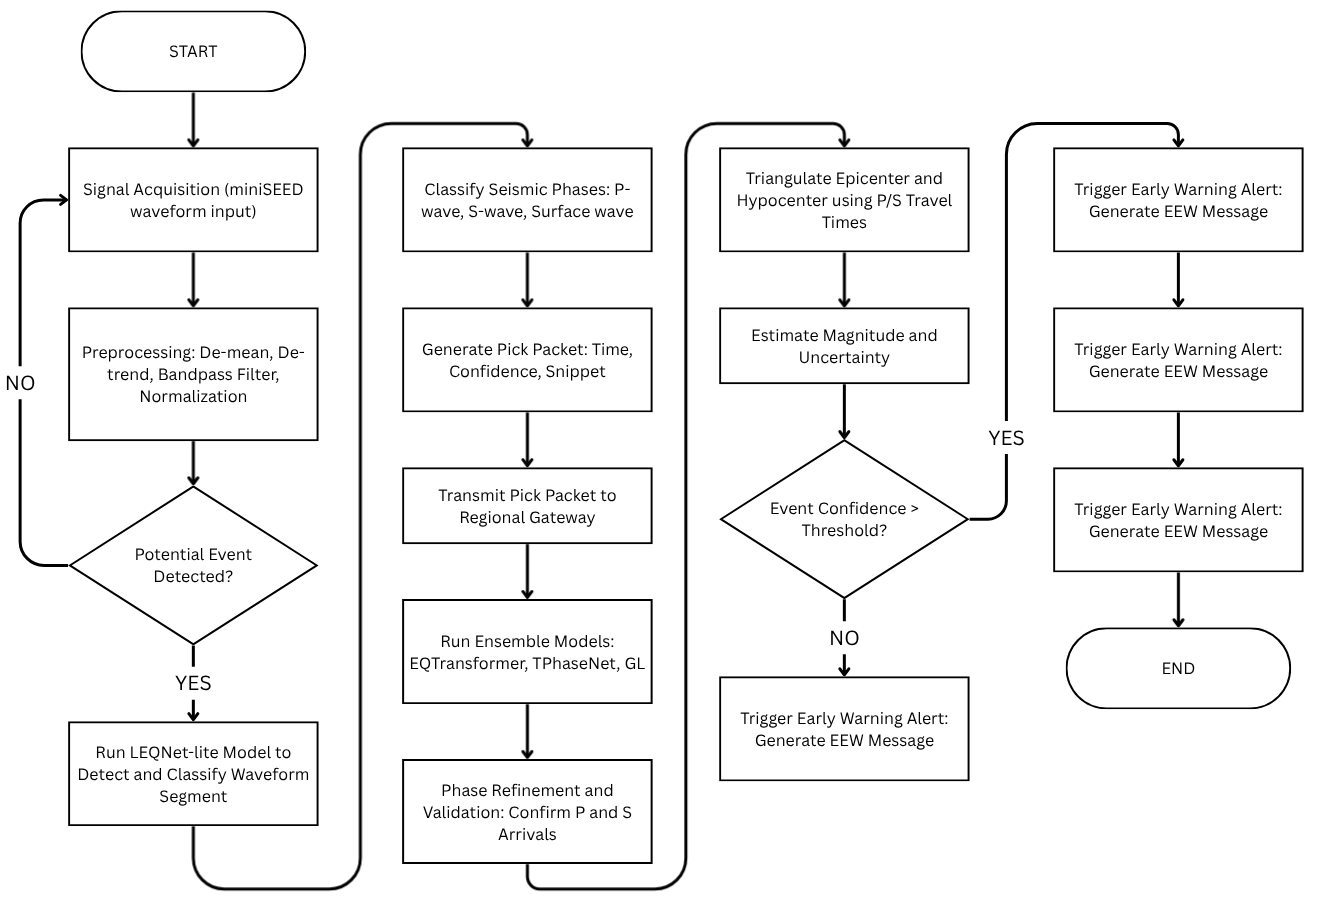
\includegraphics[width=0.95\linewidth]{operations_fl.png}
    \caption{Flow-chart representation of the SeismicQuake inference pipeline}
    \label{fig:architecture.1}
    \end{figure}

\begin{figure}[h!]
    \centering
    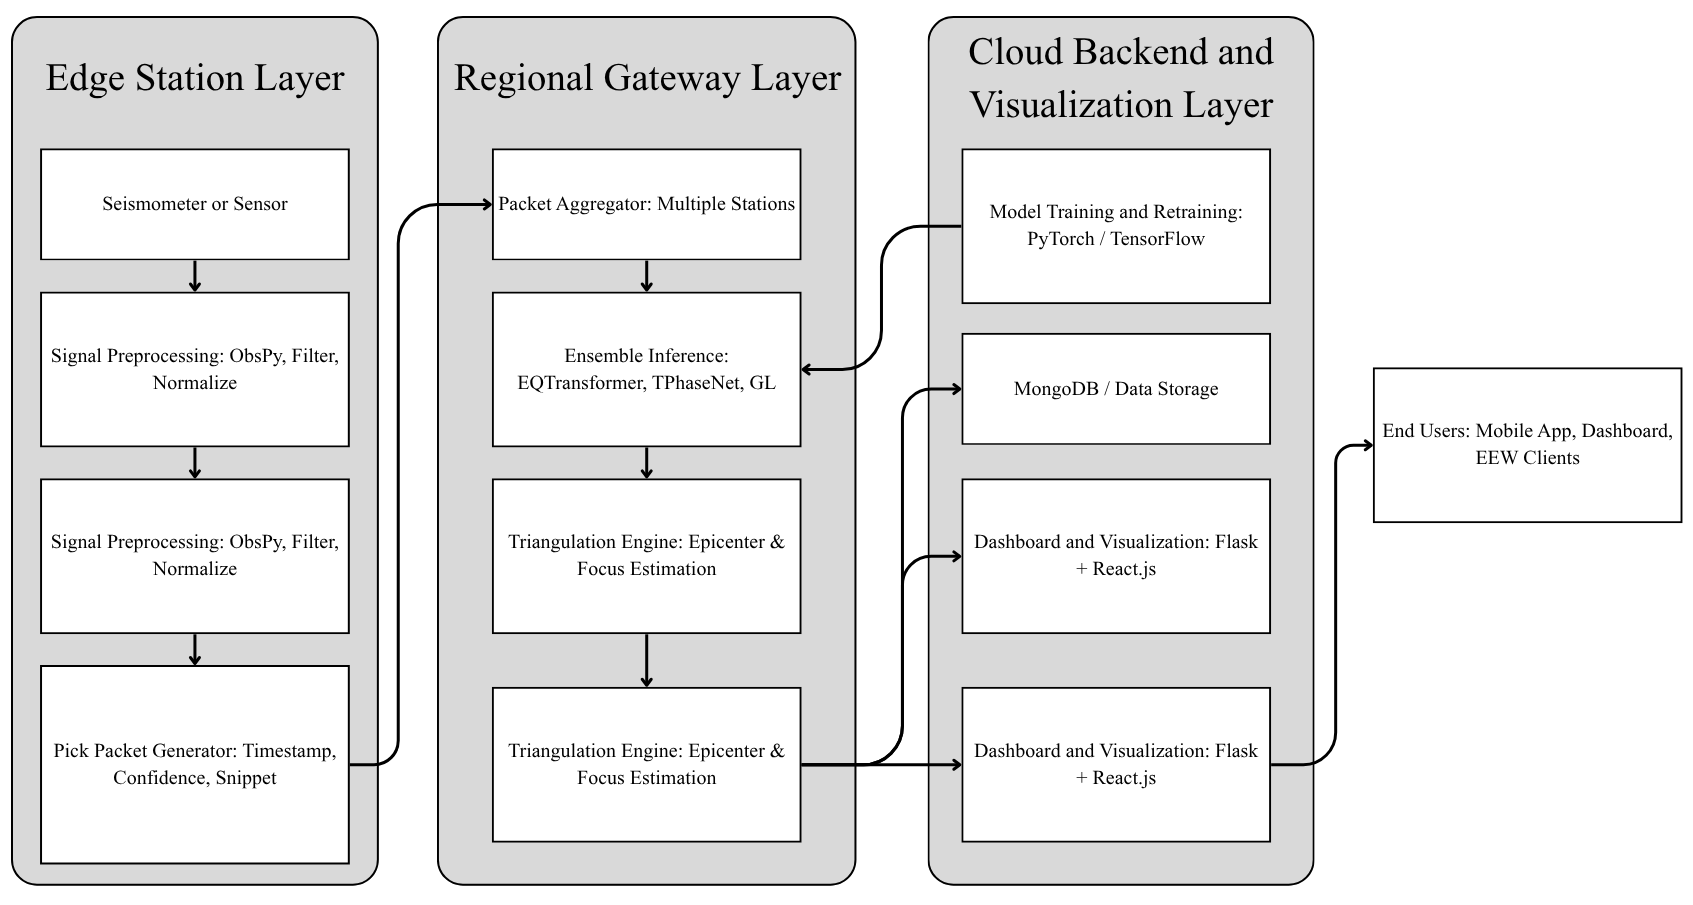
\includegraphics[width=0.95\linewidth]{systemarc_fl.png}
    \caption{System Architecture Diagram}
    \label{fig:architecture.2}
    \end{figure}

\section{Algorithms Used in the Project}
\label{sec:algorithms_used}

\subsection{1D Convolutional Neural Network (1D CNN)}
\textbf{Used in:} Earthquake Detector, Wave Classifier

\textbf{Explanation:} A 1D Convolutional Neural Network (CNN) is a deep learning algorithm designed to process time-series data, such as seismic signals. Instead of analyzing images (like 2D CNNs), it applies convolution operations along a single dimension (time axis).

\textbf{Working in this project:}
\begin{itemize}
\item Takes seismic waveform as input (amplitude vs time).
\item Applies multiple convolution layers to extract features like sudden spikes (P-wave onset) and energy variations (S-wave, surface waves).
\item Learns patterns automatically instead of using fixed thresholds.
\end{itemize}

\textbf{Why used:}
\begin{itemize}
\item Efficient for temporal signal processing.
\item Captures local patterns in seismic waves.
\item Works well for real-time detection.
\end{itemize}

\subsection{Global Average Pooling (GAP)}
\textbf{Used in:} Earthquake Detector

\textbf{Explanation:} Global Average Pooling is a technique used at the end of CNN layers to reduce data dimensions by taking the average of each feature map.

\textbf{Working in this project:}
\begin{itemize}
\item Converts feature maps into a single value per channel.
\item Reduces the number of parameters.
\item Prevents overfitting.
\end{itemize}

\textbf{Why used:}
\begin{itemize}
\item Makes the model lightweight and efficient.
\item Improves generalization on unseen data.
\end{itemize}

\subsection{Attention Mechanism}
\textbf{Used in:} Wave Classifier

\textbf{Explanation:} The Attention Mechanism is a deep learning technique that allows the model to focus on important parts of the input signal instead of treating all parts equally.

\textbf{Working in this project:}
\begin{itemize}
\item Identifies critical regions like P-wave onset and S-wave transitions.
\item Assigns higher importance (weights) to these regions.
\end{itemize}

\textbf{Why used:}
\begin{itemize}
\item Helps distinguish subtle differences between wave types.
\item Improves classification accuracy (\(\sim 99\%\) in results).
\end{itemize}

\subsection{Long Short-Term Memory (LSTM)}
\textbf{Used in:} Magnitude Predictor

\textbf{Explanation:} LSTM is a type of Recurrent Neural Network (RNN) designed to learn long-term dependencies in sequential data.

\textbf{Working in this project:}
\begin{itemize}
\item Processes time-series seismic data step-by-step.
\item Remembers important past information (wave evolution).
\item Captures how signals change over time.
\end{itemize}

\textbf{Why used:}
\begin{itemize}
\item Essential for temporal pattern understanding.
\item Improves magnitude prediction accuracy.
\end{itemize}

\subsection{Bidirectional LSTM (Bi-LSTM)}
\textbf{Used in:} Magnitude Predictor

\textbf{Explanation:} Bidirectional LSTM processes data in both forward and backward directions, giving better context.

\textbf{Working in this project:}
\begin{itemize}
\item Reads seismic signal forward (past $\rightarrow$ future) and backward (future $\rightarrow$ past).
\item Combines both insights for better prediction.
\end{itemize}

\textbf{Why used:}
\begin{itemize}
\item Captures complete temporal context.
\item Improves estimation from short signals (like 4 sec P-wave).
\end{itemize}

\subsection{Hybrid CNN-LSTM Architecture}
\textbf{Used in:} Magnitude Predictor

\textbf{Explanation:} This is a combination of CNN (feature extraction) and LSTM (sequence learning).

\textbf{Working in this project:}
\begin{itemize}
\item CNN extracts spatial features from waveform.
\item LSTM analyzes temporal dependencies.
\item Output is used for magnitude regression.
\end{itemize}

\textbf{Why used:}
\begin{itemize}
\item Combines strengths of both models.
\item Achieves low MAE (0.37) for magnitude prediction.
\end{itemize}

\subsection{Ring Buffer Algorithm}
\textbf{Used in:} Input Module (Real-time streaming)

\textbf{Explanation:} A ring buffer (circular buffer) is a data structure used to handle continuous data streams efficiently.

\textbf{Working in this project:}
\begin{itemize}
\item Stores fixed-size recent seismic data.
\item New data overwrites old data.
\item Ensures continuous real-time input.
\end{itemize}

\textbf{Why used:}
\begin{itemize}
\item Enables real-time processing.
\item Prevents memory overflow.
\item Maintains latest signal window.
\end{itemize}

\subsection{Data Preprocessing Techniques (Supporting Algorithms)}
These are not single algorithms but important steps:

\paragraph{a) Normalization}
Scales waveform to range [-1, 1]. Ensures stable training.

\paragraph{b) Windowing}
Splits signal into 4-second segments (400 samples). Helps model learn local patterns.

\paragraph{c) Class Balancing}
Assigns weights to handle imbalance between noise and earthquake data.

\subsection{STA/LTA Trigger Algorithm (Short-Term Average / Long-Term Average)}
\label{ssec:stalta_baseline}

\textbf{Used in:} Existing traditional seismic detection systems (baseline comparison).

\textbf{Explanation:} The STA/LTA (Short-Term Average / Long-Term Average) Trigger algorithm is a classical signal processing technique used for earthquake detection. It works by comparing the short-term energy of a seismic signal with its long-term average energy to identify sudden changes that indicate seismic events.

\textbf{Working Principle:}
The algorithm computes two moving averages over the seismic signal:
\begin{itemize}
\item \textbf{Short-Term Average (STA):} Calculated over a small time window (captures sudden signal changes).
\item \textbf{Long-Term Average (LTA):} Calculated over a larger time window (represents background noise level).
\end{itemize}

The ratio is then computed as:
\[
\text{Trigger Ratio}=\frac{\text{STA}}{\text{LTA}}
\]

If the ratio exceeds a predefined threshold, an earthquake event is detected; otherwise, the signal is considered noise.

\textbf{Working in Seismic Systems:}
\begin{itemize}
\item Continuously monitor incoming seismic signal.
\item Compute STA and LTA in real-time.
\item Detect sudden increases in signal energy.
\item Trigger an alert when threshold is crossed.
\end{itemize}

\textbf{Advantages:}
\begin{itemize}
\item Simple and easy to implement.
\item Low computational cost.
\item Works reasonably well for clear seismic signals.
\end{itemize}

\section{SAMPLE CODES}
\label{sec:sample_codes}

The following sample codes represent key implementation blocks used in SeismicQuake.

\subsection{Waveform Preprocessing}

\begin{lstlisting}[language=Python, caption={Signal loading and preprocessing}, basicstyle=\ttfamily\small, breaklines=true]
import numpy as np
from obspy import read
from scipy.signal import butter, filtfilt

def bandpass_filter(x, fs=100, low=1.0, high=20.0, order=4):
    nyq = 0.5 * fs
    b, a = butter(order, [low / nyq, high / nyq], btype="band")
    return filtfilt(b, a, x)

def preprocess_mseed(path, window_size=400):
    st = read(path)
    tr = st[0]  # vertical component can also be selected explicitly
    x = tr.data.astype(np.float32)

    # de-mean + detrend
    x = x - np.mean(x)
    x = x - np.linspace(x[0], x[-1], len(x))

    # filtering + normalization
    x = bandpass_filter(x, fs=int(tr.stats.sampling_rate))
    x = x / (np.max(np.abs(x)) + 1e-8)

    # split into 4-second windows (400 samples at 100 Hz)
    windows = []
    for i in range(0, len(x) - window_size + 1, window_size):
        windows.append(x[i:i + window_size])
    return np.array(windows, dtype=np.float32)
\end{lstlisting}

\subsection{Earthquake Detector (1D-CNN)}

\begin{lstlisting}[language=Python, caption={Binary earthquake detector model}, basicstyle=\ttfamily\small, breaklines=true]
from tensorflow.keras import Sequential
from tensorflow.keras.layers import Conv1D, MaxPooling1D, BatchNormalization
from tensorflow.keras.layers import GlobalAveragePooling1D, Dense, Dropout

def build_detector(input_shape=(400, 1)):
    model = Sequential([
        Conv1D(32, 7, activation="relu", padding="same", input_shape=input_shape),
        BatchNormalization(), MaxPooling1D(2),
        Conv1D(64, 5, activation="relu", padding="same"),
        BatchNormalization(), MaxPooling1D(2),
        Conv1D(128, 3, activation="relu", padding="same"),
        BatchNormalization(), MaxPooling1D(2),
        Conv1D(256, 3, activation="relu", padding="same"),
        BatchNormalization(),
        GlobalAveragePooling1D(),
        Dropout(0.3),
        Dense(128, activation="relu"),
        Dropout(0.3),
        Dense(64, activation="relu"),
        Dense(1, activation="sigmoid")
    ])
    model.compile(optimizer="adam", loss="binary_crossentropy", metrics=["accuracy"])
    return model
\end{lstlisting}

\subsection{Wave Classifier (1D-CNN with Attention)}

\begin{lstlisting}[language=Python, caption={Wave phase classifier with attention}, basicstyle=\ttfamily\small, breaklines=true]
import tensorflow as tf
from tensorflow.keras.layers import Input, Conv1D, MaxPooling1D, BatchNormalization
from tensorflow.keras.layers import Multiply, GlobalAveragePooling1D, Dropout, Dense
from tensorflow.keras.models import Model

def build_wave_classifier(input_shape=(400, 1), n_classes=3):
    inp = Input(shape=input_shape)
    x = Conv1D(32, 7, activation="relu", padding="same")(inp)
    x = BatchNormalization()(x); x = MaxPooling1D(2)(x)
    x = Conv1D(64, 5, activation="relu", padding="same")(x)
    x = BatchNormalization()(x); x = MaxPooling1D(2)(x)
    x = Conv1D(128, 3, activation="relu", padding="same")(x)
    x = BatchNormalization()(x); x = MaxPooling1D(2)(x)

    attn = Conv1D(1, 1, activation="sigmoid", padding="same")(x)
    x = Multiply()([x, attn])

    x = Conv1D(256, 3, activation="relu", padding="same")(x)
    x = BatchNormalization()(x)
    x = GlobalAveragePooling1D()(x)
    x = Dropout(0.4)(x)
    x = Dense(128, activation="relu")(x)
    x = Dropout(0.3)(x)
    x = Dense(64, activation="relu")(x)
    out = Dense(n_classes, activation="softmax")(x)

    model = Model(inp, out)
    model.compile(optimizer="adam",
                  loss="categorical_crossentropy",
                  metrics=["accuracy"])
    return model
\end{lstlisting}

\subsection{Magnitude Predictor (Hybrid CNN-BiLSTM)}

\begin{lstlisting}[language=Python, caption={Magnitude regression model}, basicstyle=\ttfamily\small, breaklines=true]
from tensorflow.keras.layers import Bidirectional, LSTM

def build_magnitude_model(input_shape=(400, 1)):
    inp = Input(shape=input_shape)
    x = Conv1D(32, 7, activation="relu", padding="same")(inp)
    x = BatchNormalization()(x); x = MaxPooling1D(2)(x)
    x = Conv1D(64, 5, activation="relu", padding="same")(x)
    x = BatchNormalization()(x); x = MaxPooling1D(2)(x)
    x = Conv1D(128, 3, activation="relu", padding="same")(x)
    x = BatchNormalization()(x); x = MaxPooling1D(2)(x)
    x = Conv1D(256, 3, activation="relu", padding="same")(x)
    x = BatchNormalization()(x)

    x = Bidirectional(LSTM(64))(x)
    x = Dropout(0.4)(x)
    x = Dense(128, activation="relu")(x)
    x = Dropout(0.3)(x)
    x = Dense(64, activation="relu")(x)
    x = Dense(32, activation="relu")(x)
    out = Dense(1, activation="linear")(x)

    model = Model(inp, out)
    model.compile(optimizer="adam", loss="mse", metrics=["mae"])
    return model
\end{lstlisting}

\subsection{Sequential Inference Pipeline}

\begin{lstlisting}[language=Python, caption={End-to-end analysis flow}, basicstyle=\ttfamily\small, breaklines=true]
WAVE_LABELS = ["P-wave", "S-wave", "Surface-wave"]

def analyze_window(window, detector, classifier, magnitude_model, det_th=0.5):
    x = window.reshape(1, 400, 1).astype("float32")

    # Stage 1: event detection
    det_prob = float(detector.predict(x, verbose=0)[0][0])
    if det_prob < det_th:
        return {"event": False, "confidence": det_prob}

    # Stage 2: phase classification
    phase_prob = classifier.predict(x, verbose=0)[0]
    phase_idx = int(np.argmax(phase_prob))
    phase_name = WAVE_LABELS[phase_idx]

    result = {
        "event": True,
        "confidence": det_prob,
        "wave_type": phase_name,
        "wave_score": float(np.max(phase_prob))
    }

    # Stage 3: magnitude estimation (optional for P-wave windows)
    if phase_name == "P-wave":
        mag = float(magnitude_model.predict(x, verbose=0)[0][0])
        result["magnitude"] = round(mag, 2)

    return result
\end{lstlisting}

\newpage


% --- CHAPTER 4 ---
\chapter{RESULTS}
\label{sec:chapter4_result_images}

\section{Performance Summary}
\label{sec:chapter4_performance_summary}

\textbf{Earthquake Detection}
\begin{itemize}
\item \textbf{Accuracy:} 96.81\%
\item \textbf{AUC-ROC:} 99.59\%
\end{itemize}

The high AUC score indicates the model is extremely effective at ranking earthquake signals higher than noise, even at low false positive rates.

\vspace{0.3cm}
\textbf{Wave Classification (Multi-class)}
\begin{itemize}
\item \textbf{Overall Accuracy:} 99.69\%
\item \textbf{Per-Class Accuracy:}
  \begin{itemize}
  \item P-wave: \(\sim\)99\%
  \item S-wave: \(\sim\)99\%
  \item Surface wave: \(\sim\)99\%
  \end{itemize}
\end{itemize}

The attention mechanism proved crucial here, allowing the model to distinguish the subtle onset of P-waves from the higher-amplitude S-waves.

\vspace{0.3cm}
\textbf{Magnitude Prediction (Hybrid Deep Learning)}
\begin{itemize}
\item \textbf{Mean Absolute Error (MAE):} 0.37
\item \textbf{Within \(\pm 0.5\) Magnitude:} 75.0\%
\item \textbf{Within \(\pm 1.0\) Magnitude:} 93.1\%
\end{itemize}

Estimating magnitude from just 4 seconds of P-wave data is challenging. An MAE of 0.37 is a strong result, providing a reliable \enquote{ballpark} estimate for early warning purposes before the full seismic event has concluded.

\begin{figure}[h!]
\centering
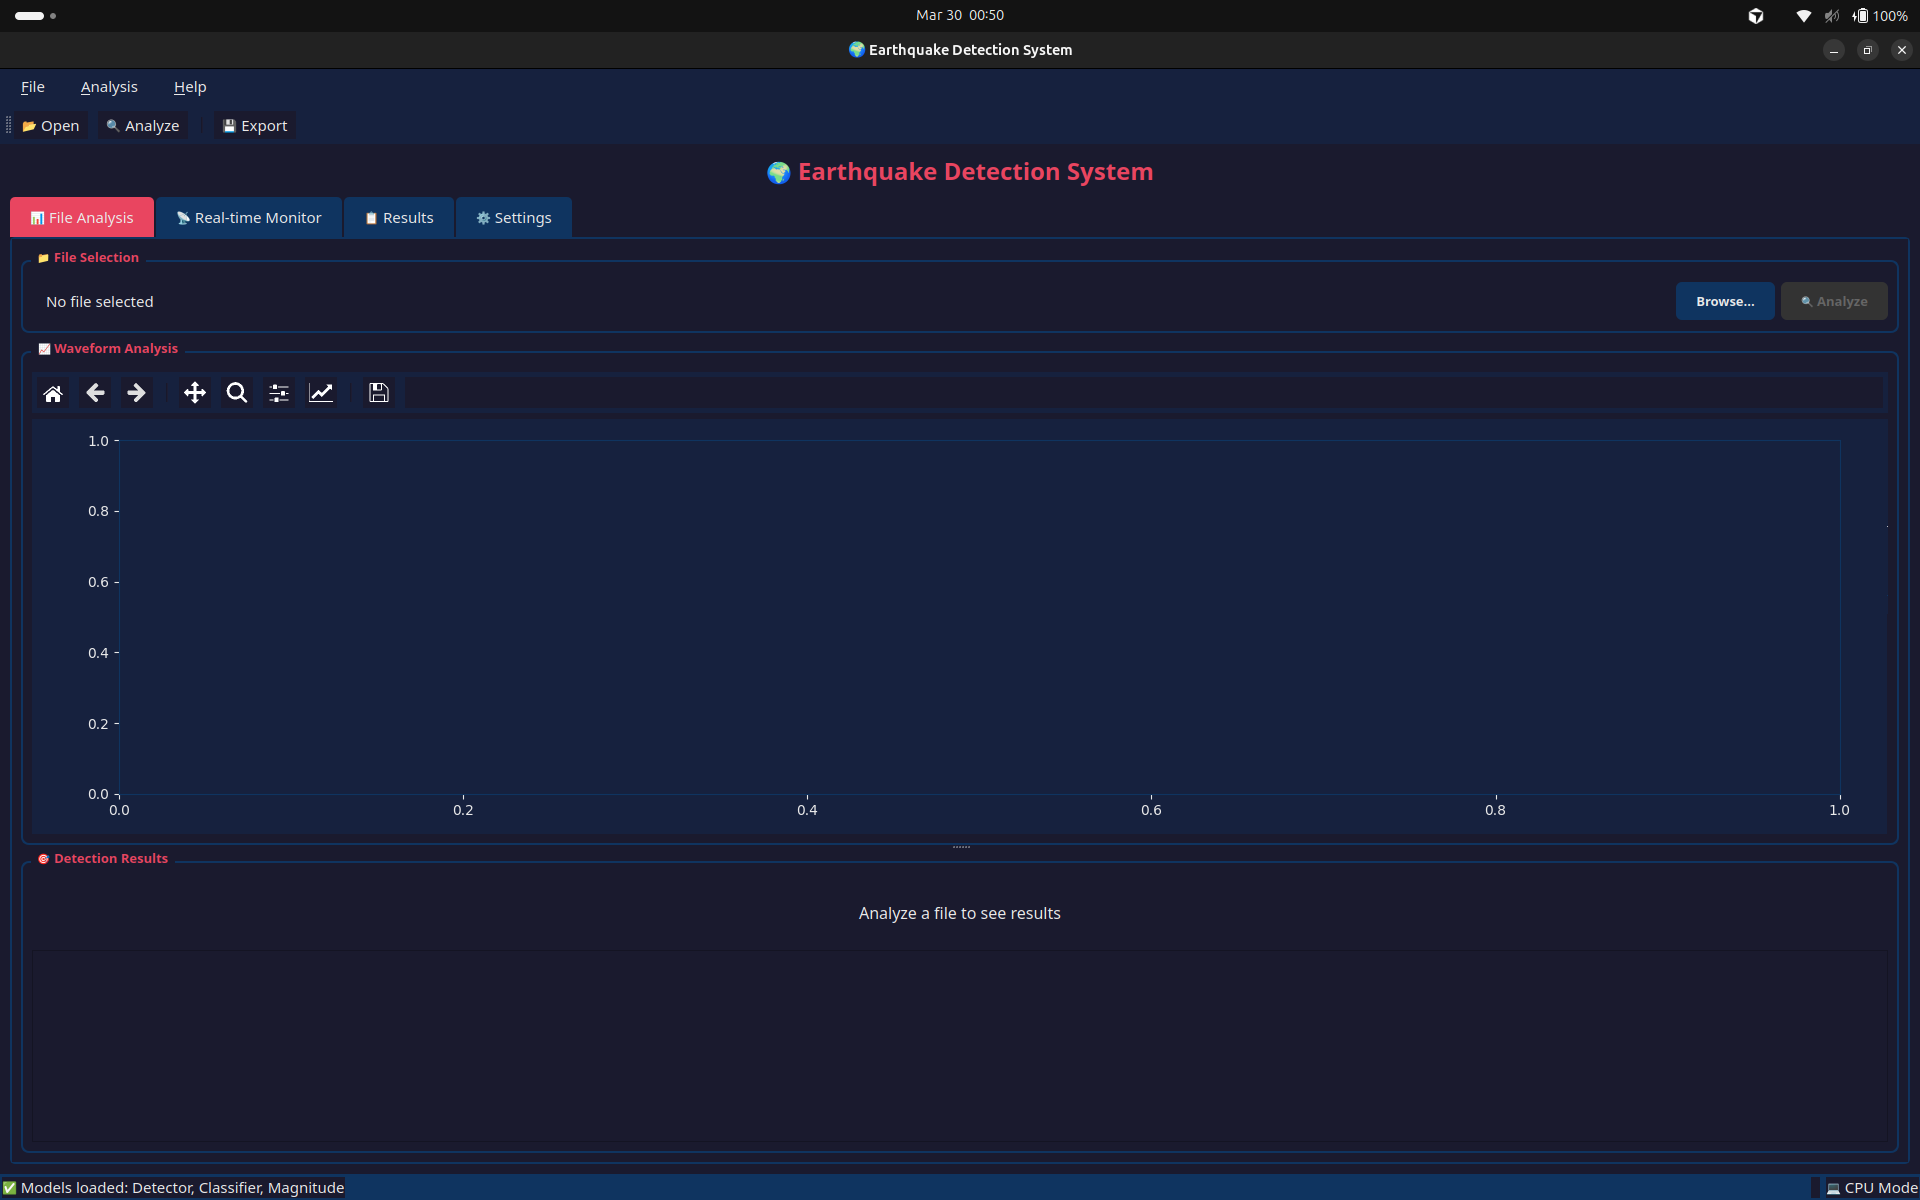
\includegraphics[width=0.95\linewidth]{images/1.png}
\caption{UI/UX Interface}
\label{fig:4.result.1}
\end{figure}

\begin{figure}[h!]
\centering
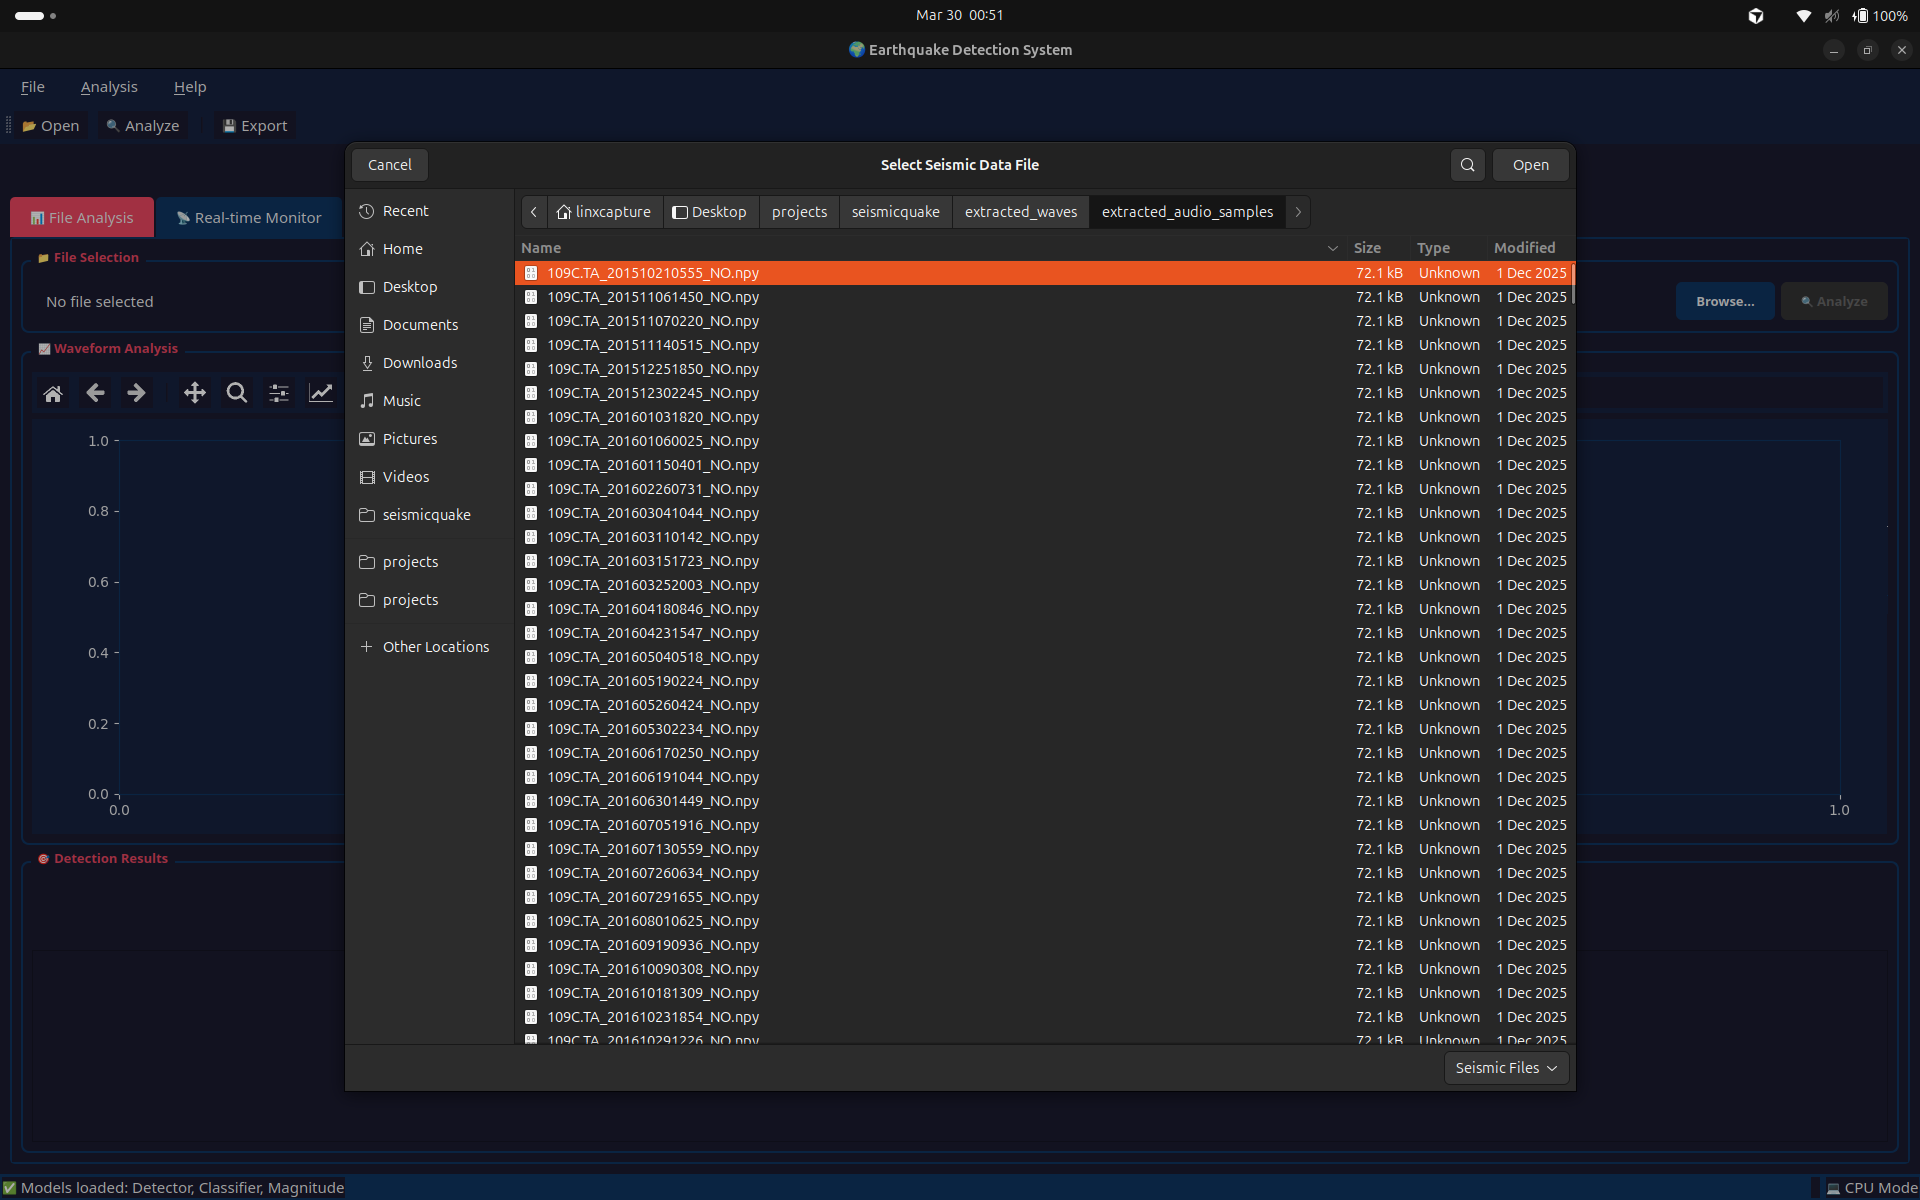
\includegraphics[width=0.95\linewidth]{images/2.png}
\caption{No Earthquake Dataset Retrived.}
\label{fig:4.result.2}
\end{figure}

\begin{figure}[h!]
\centering
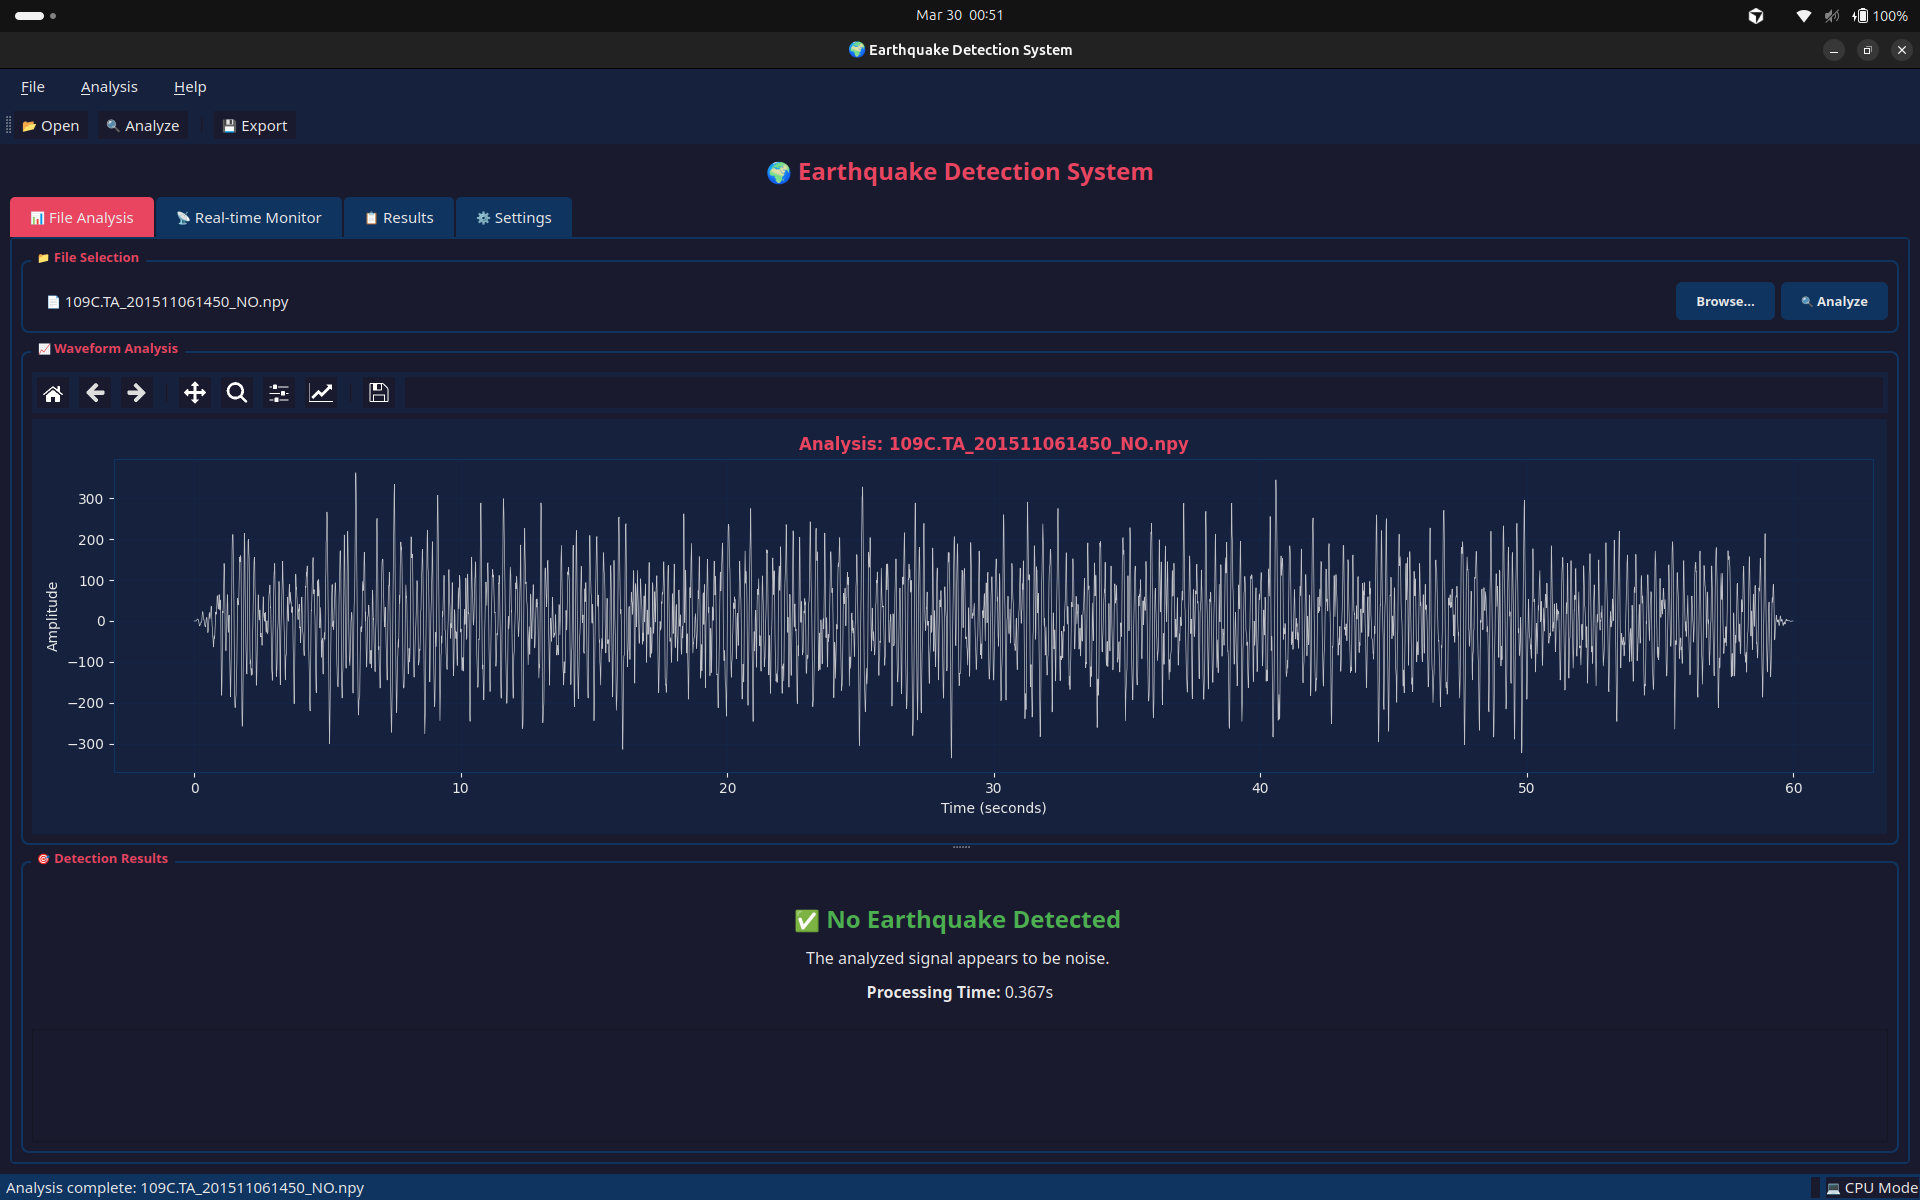
\includegraphics[width=0.95\linewidth]{images/3.png}
\caption{No Earthquake Detected}
\label{fig:4.result.3}
\end{figure}

\begin{figure}[h!]
\centering
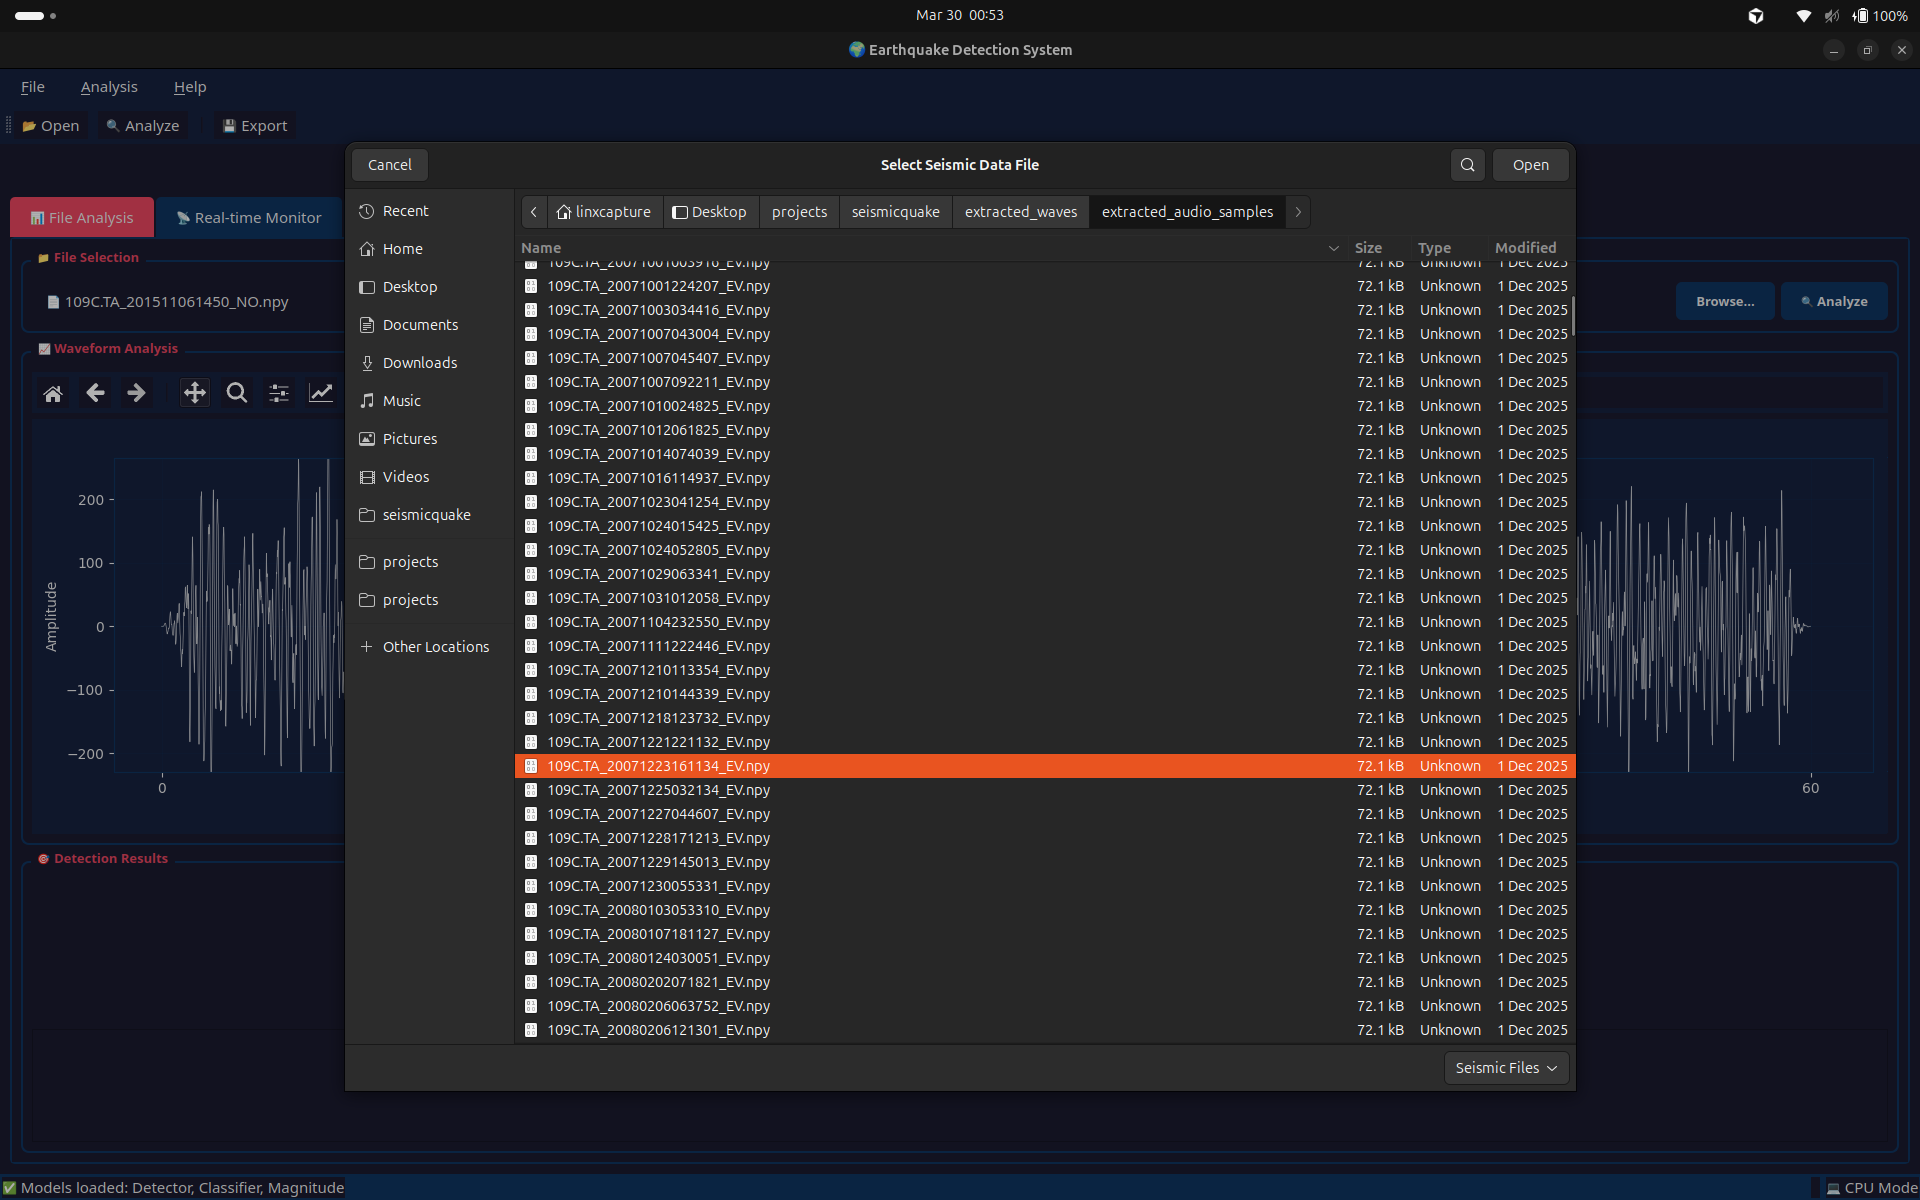
\includegraphics[width=0.95\linewidth]{images/4.png}
\caption{Earthquake Dataset Retrived.}
\label{fig:4.result.4}
\end{figure}

\begin{figure}[h!]
\centering
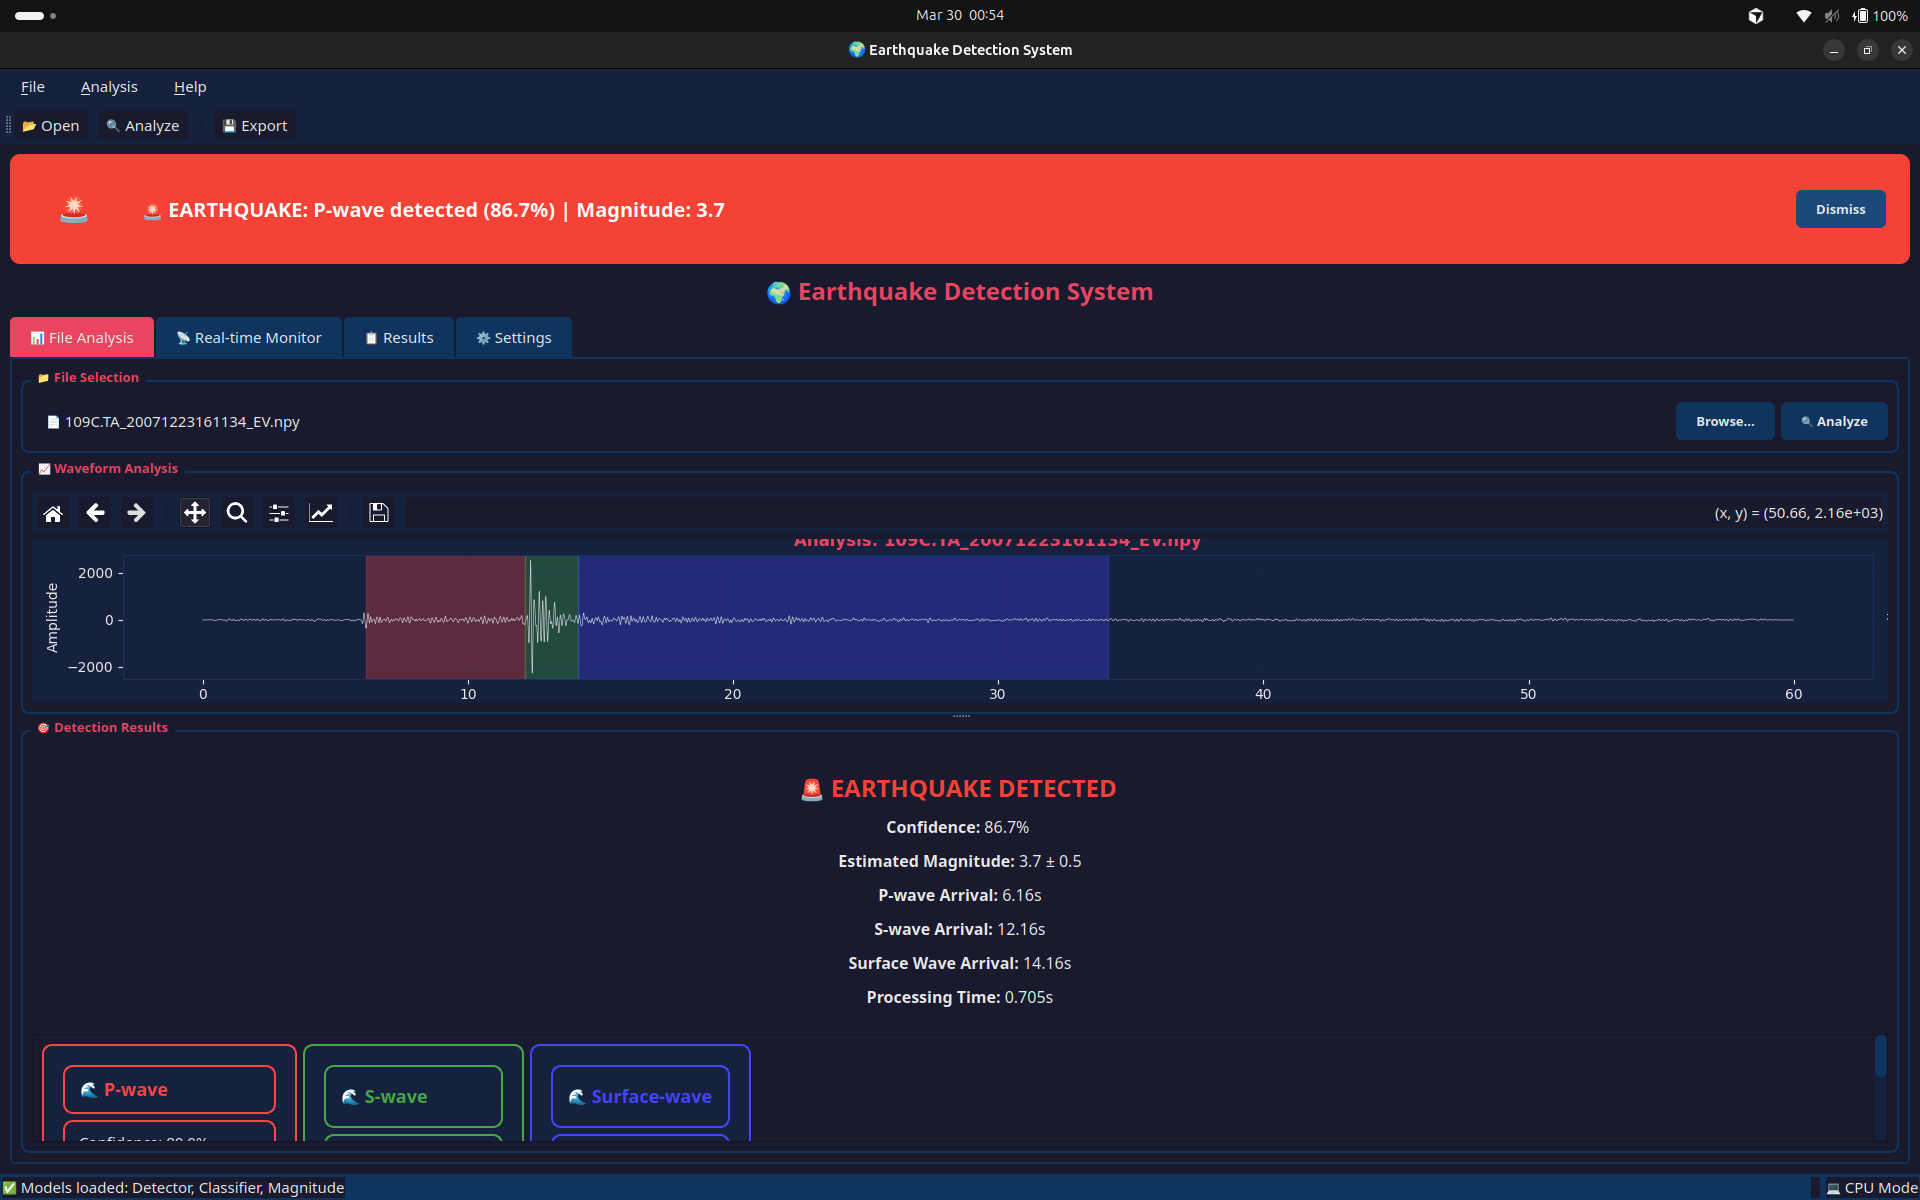
\includegraphics[width=0.95\linewidth]{images/5.png}
\caption{Earthquake Detected.}
\label{fig:4.result.5}
\end{figure}

\begin{figure}[h!]
\centering
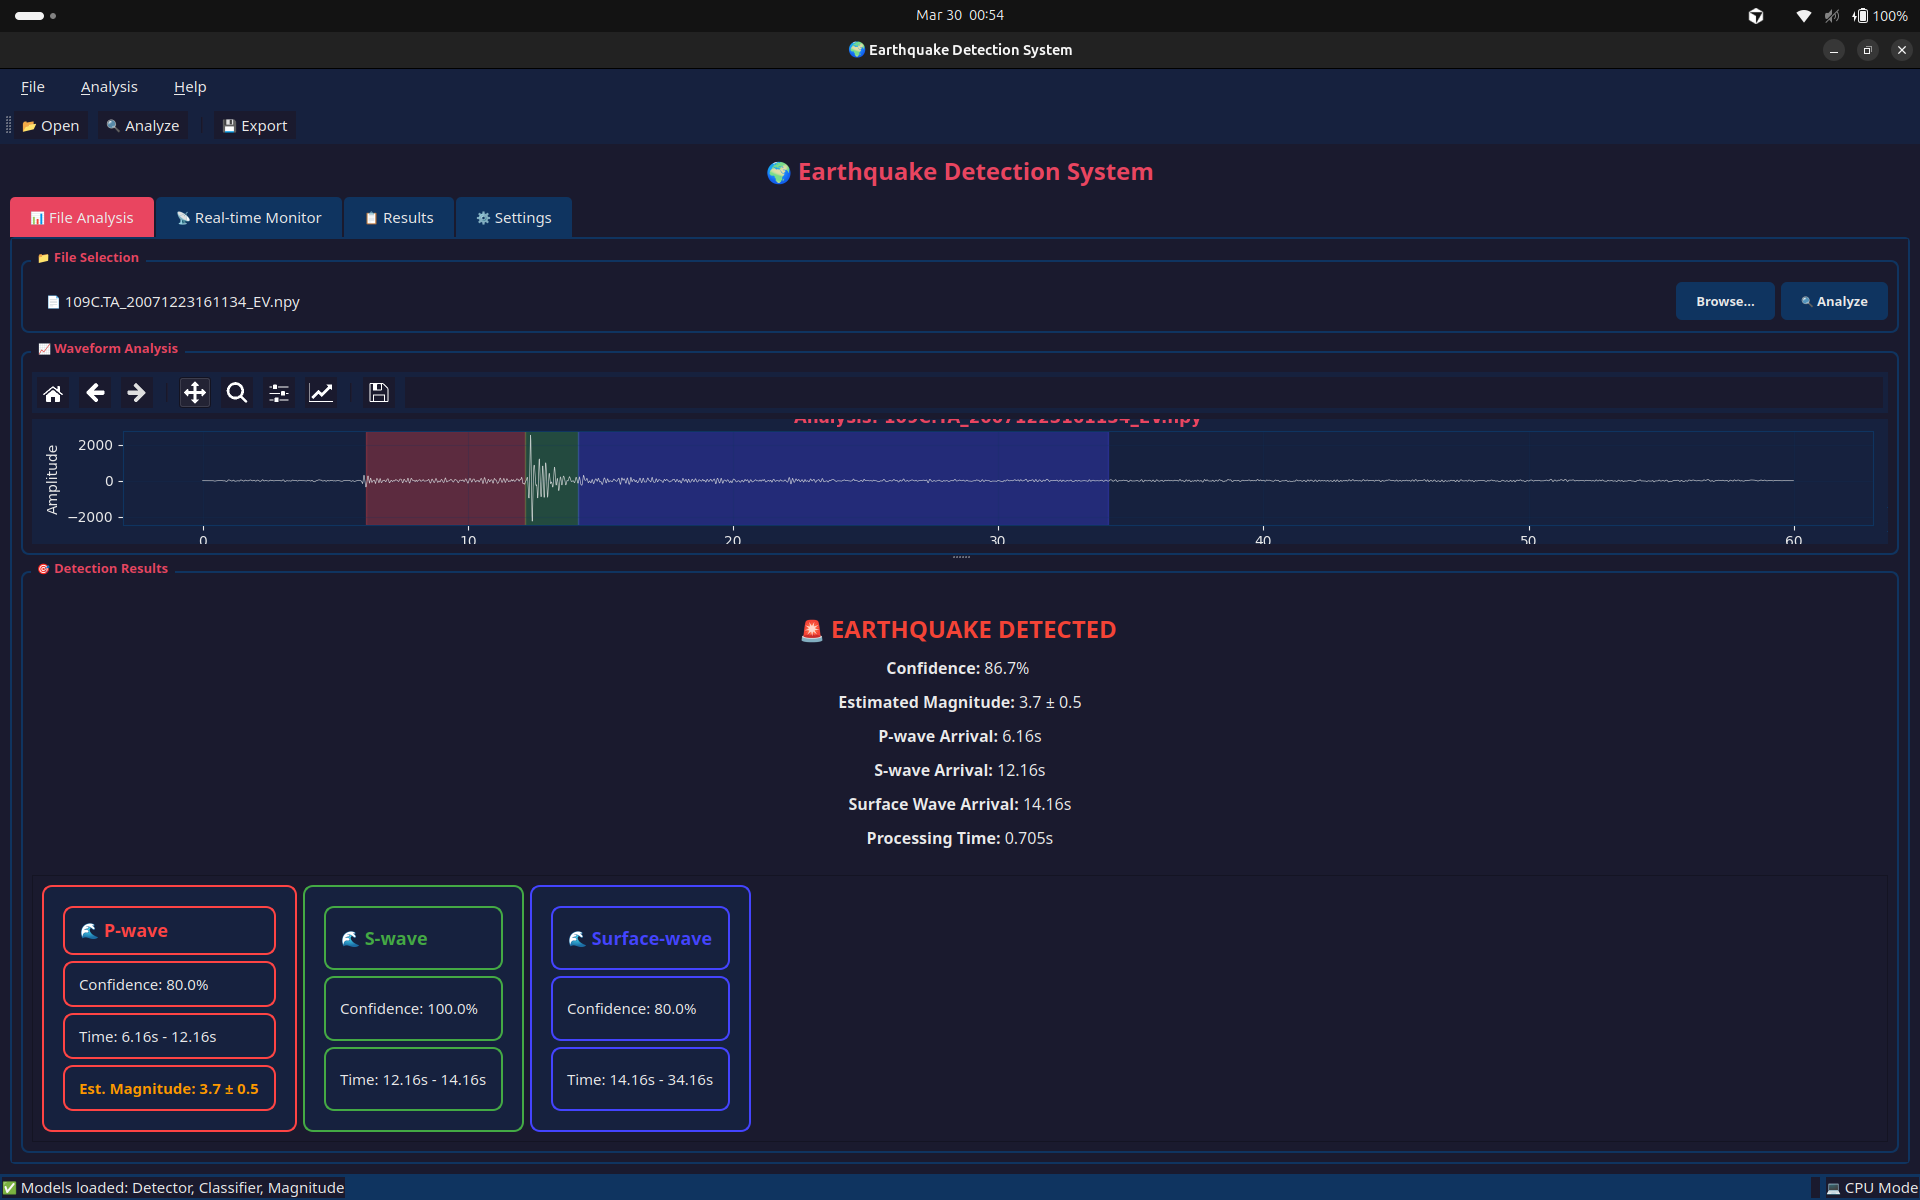
\includegraphics[width=0.95\linewidth]{images/6.png}
\caption{Types of Waves Shown.}
\label{fig:4.result.6}
\end{figure}

\begin{figure}[h!]
\centering
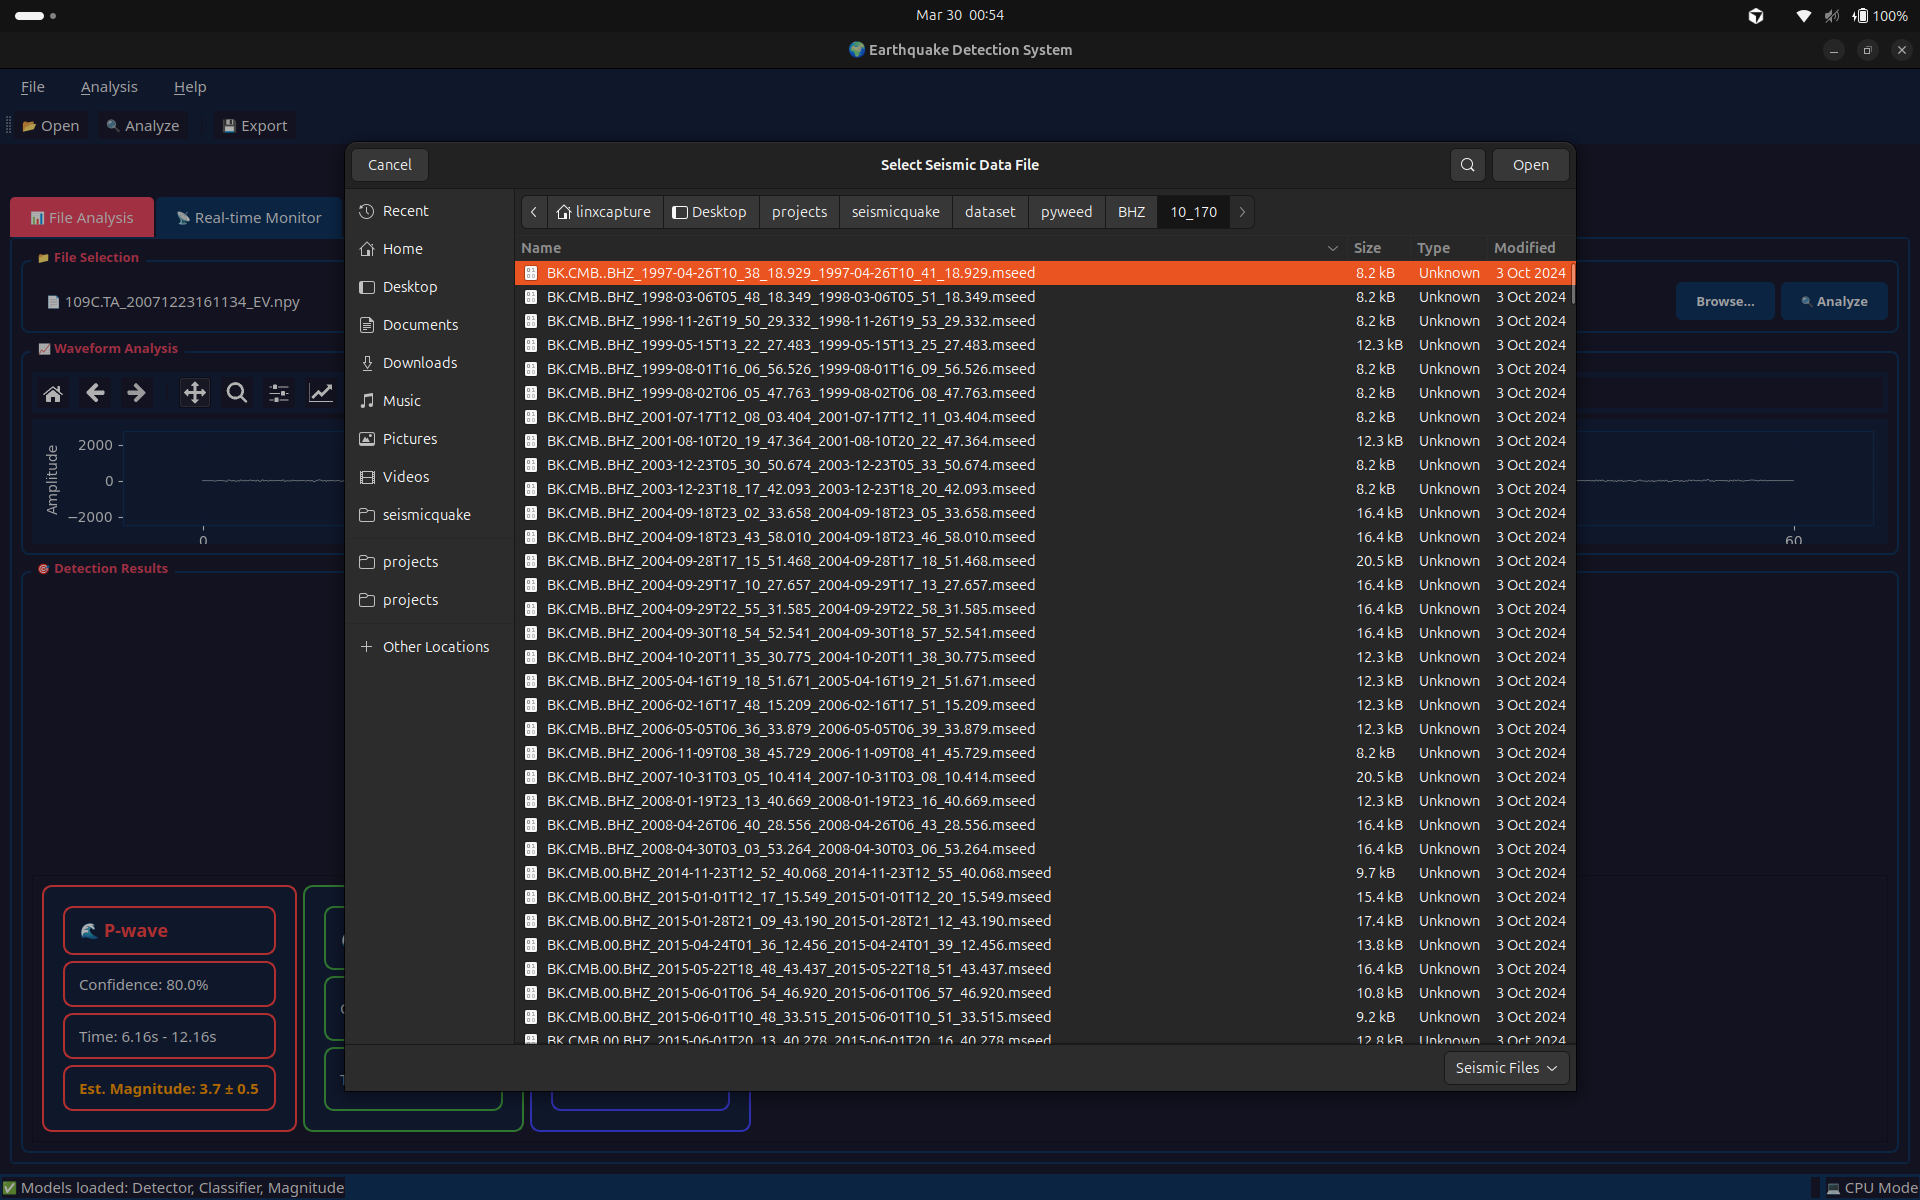
\includegraphics[width=0.95\linewidth]{images/7.png}
\caption{Magnitude Predictor Dataset.}
\label{fig:4.result.7}
\end{figure}

\begin{figure}[h!]
\centering
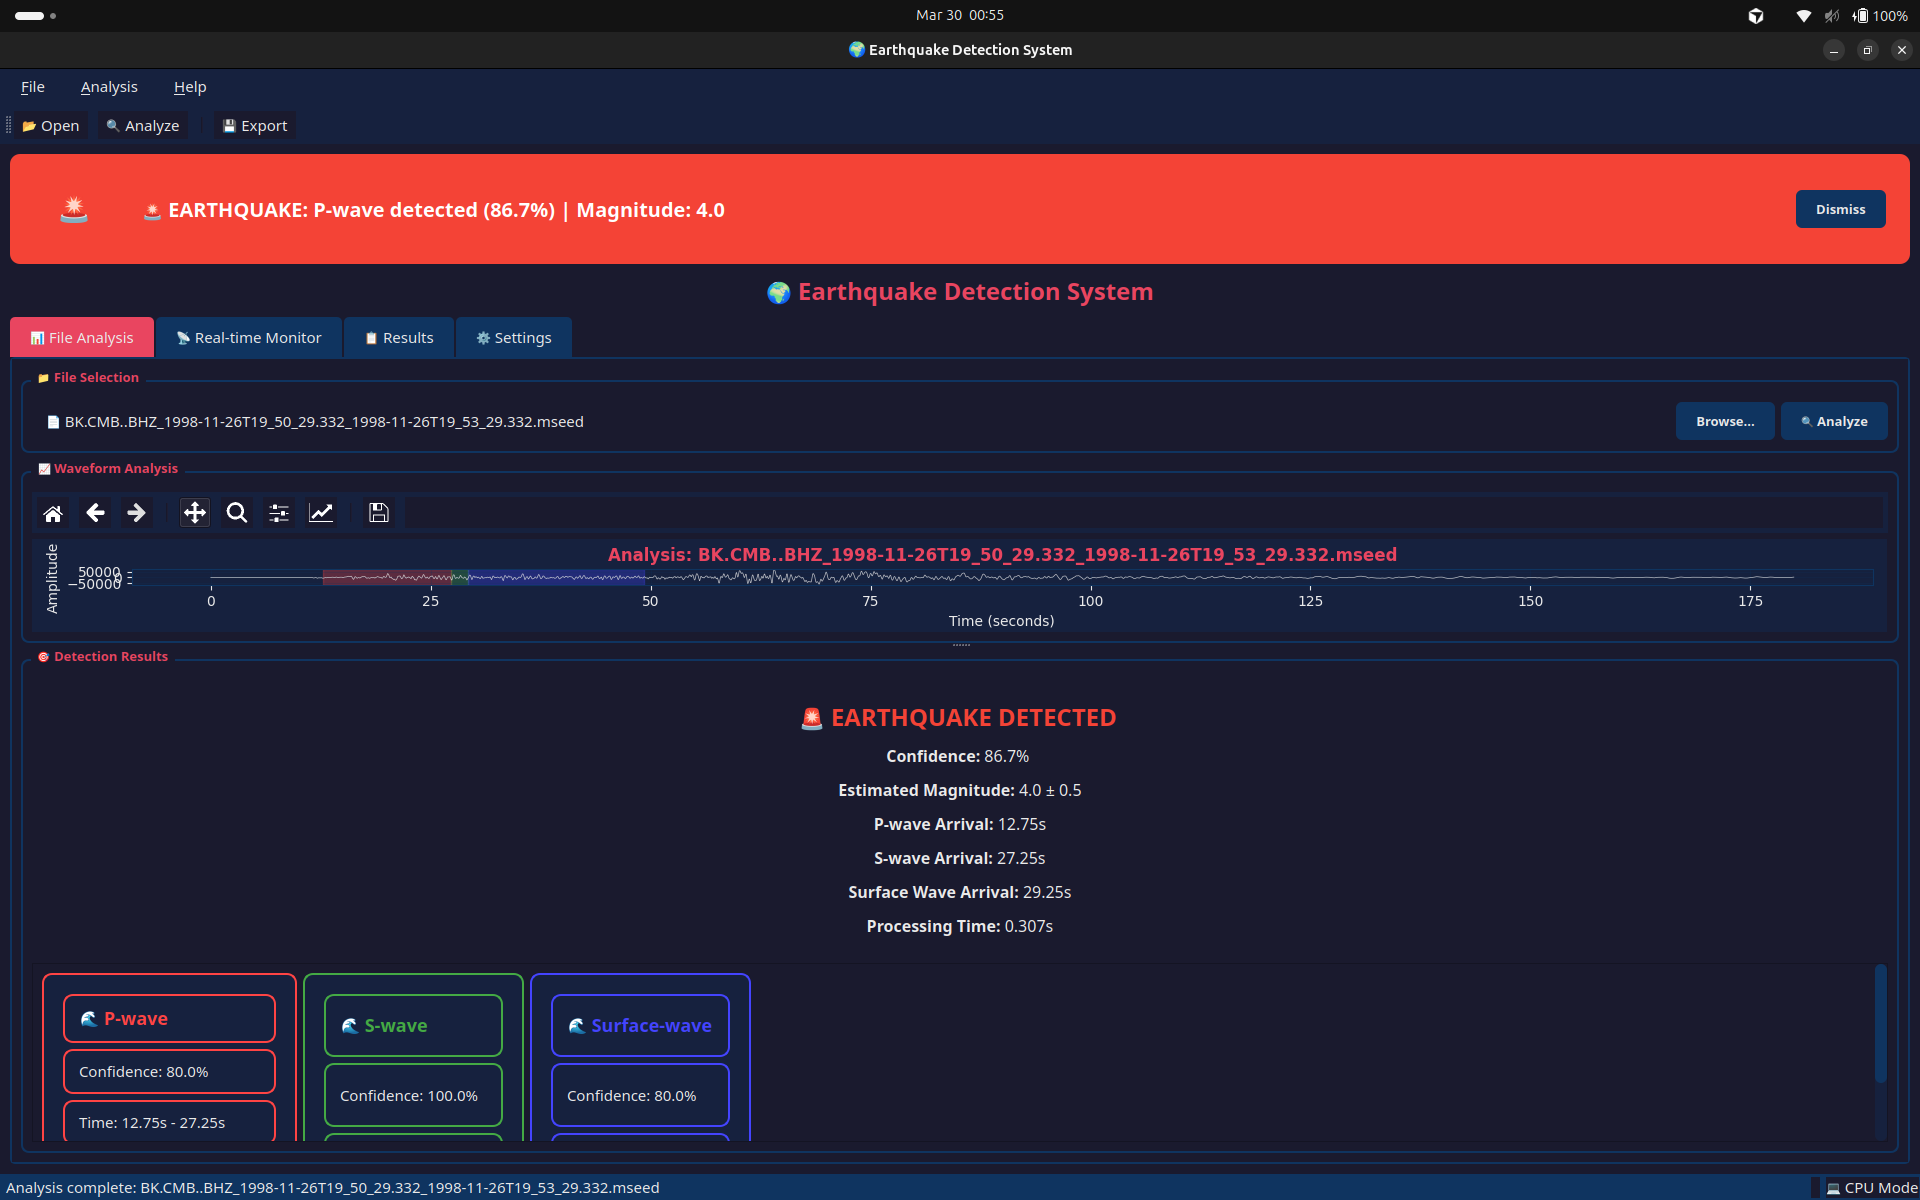
\includegraphics[width=0.95\linewidth]{images/8.png}
\caption{Magnitude Predicted.}
\label{fig:4.result.8}
\end{figure}

\begin{figure}[h!]
\centering
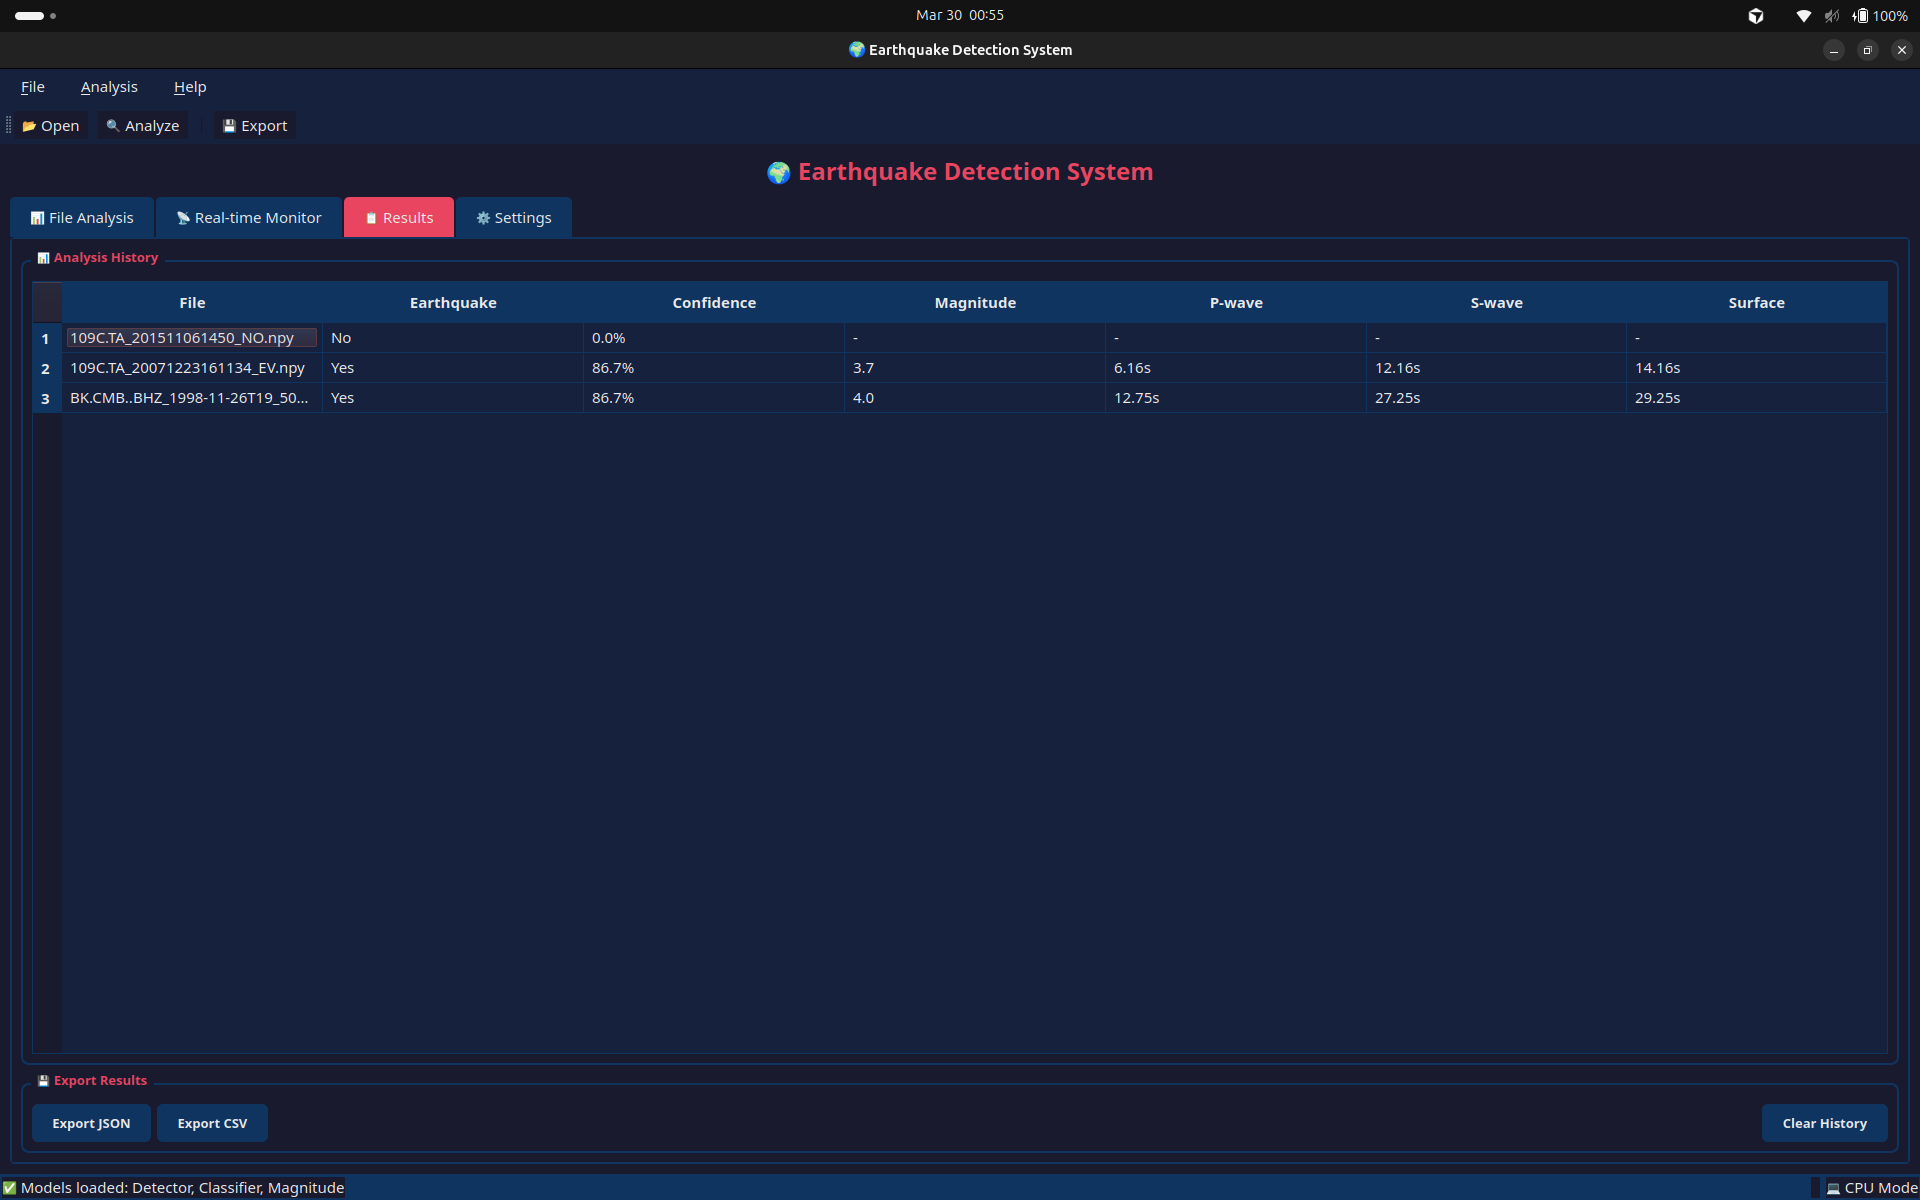
\includegraphics[width=0.95\linewidth]{images/9.png}
\caption{History of Datasets.}
\label{fig:4.result.9}
\end{figure}

\begin{figure}[h!]
\centering
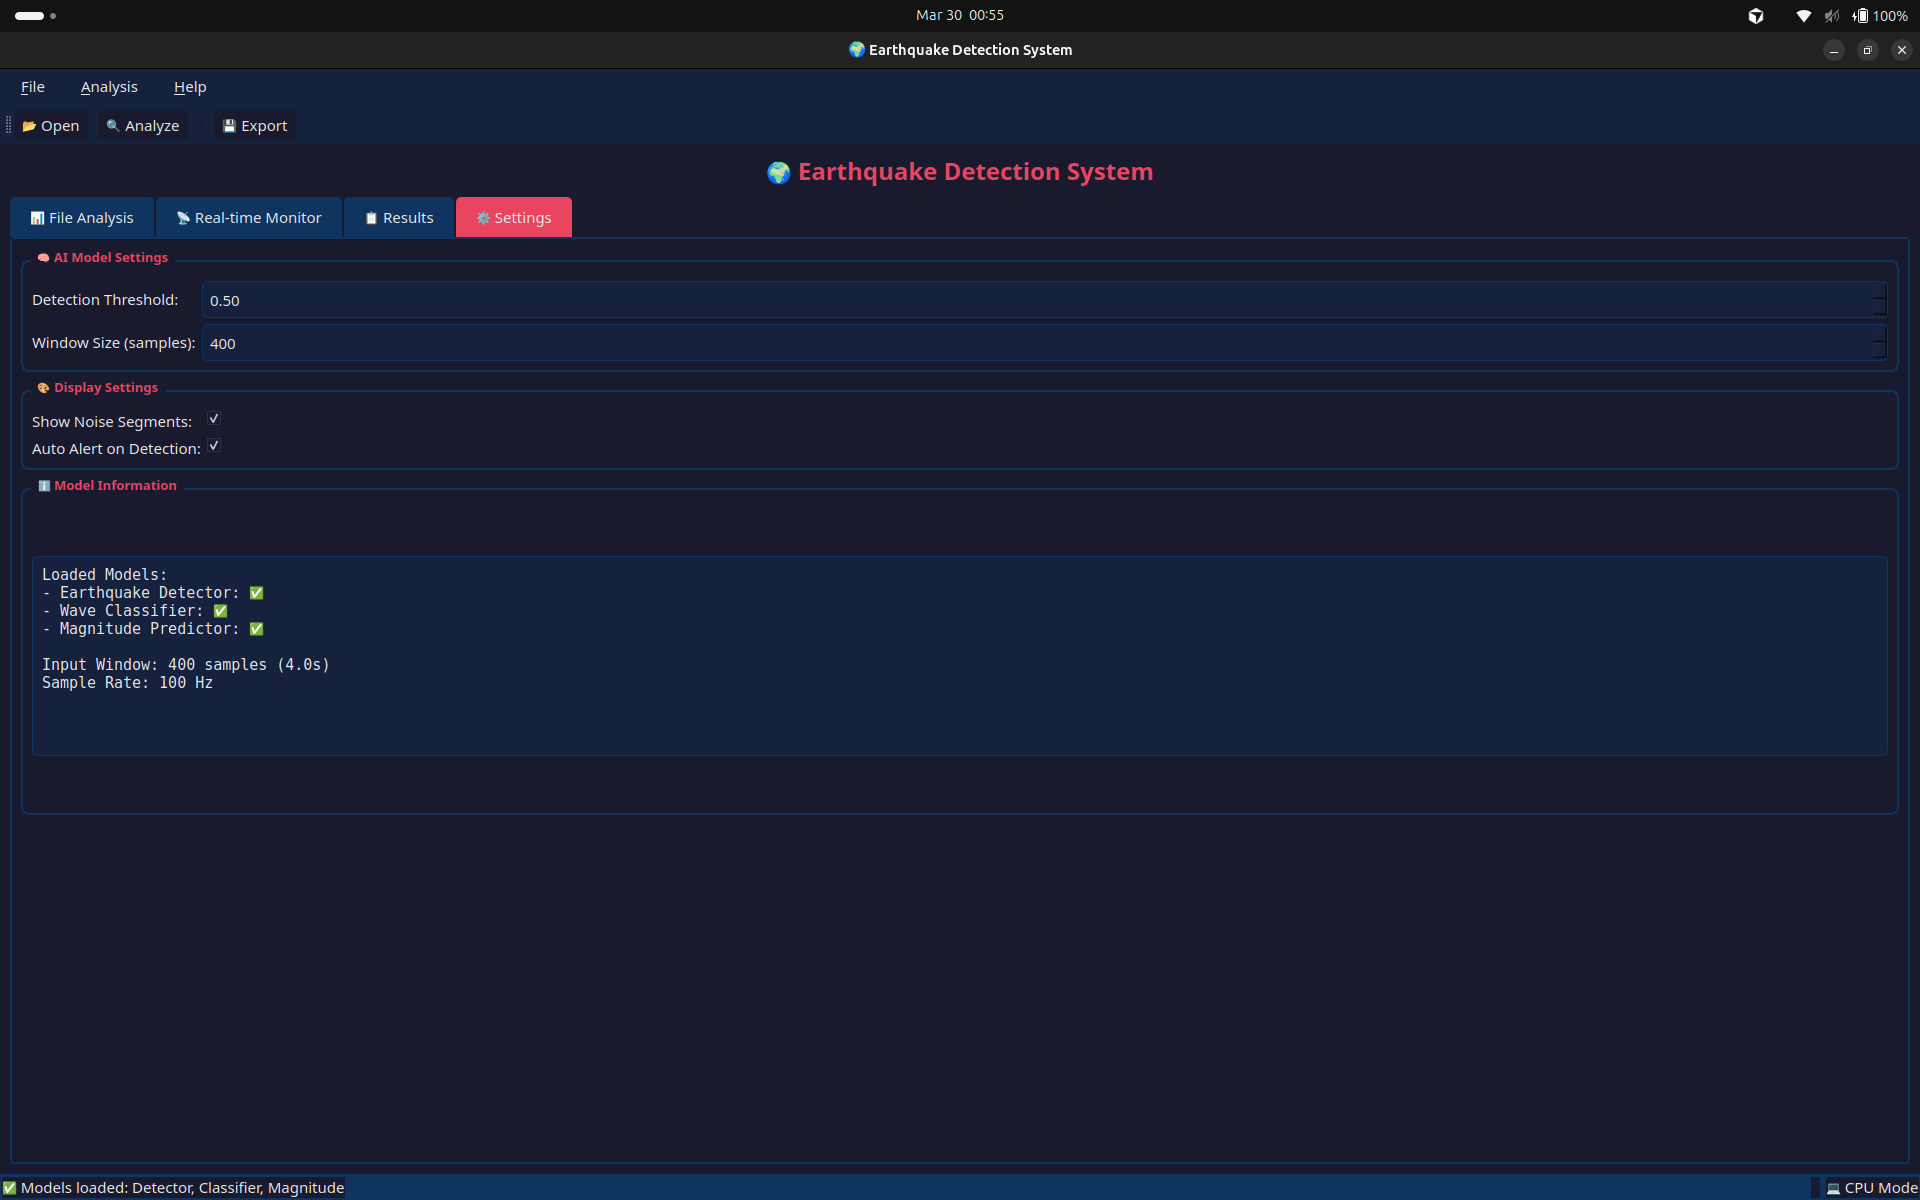
\includegraphics[width=0.95\linewidth]{images/10.png}
\caption{History of Earthquakes.}
\label{fig:4.result.10}
\end{figure}

% --- CHAPTER 5 ---
\chapter{FUTURE SCOPE}
\label{chap:future_scope}

\section{Distributed Sensing}
\label{sec:5.1}

The proposed system can be extended by incorporating distributed sensing techniques, where multiple seismic sensors are deployed across different geographic locations. Instead of relying on a single station, the system will use consensus-based algorithms to combine data from multiple sensors.

By analyzing signals from geographically dispersed nodes:
\begin{itemize}
\item The system can achieve more accurate epicenter localization.
\item It can reduce errors caused by local noise or faulty sensors.
\item It can improve reliability through cross-verification of detected events.
\end{itemize}

This approach is particularly useful for large-scale seismic monitoring networks, where coordinated sensing enhances both precision and robustness.

\section{Edge AI Deployment}
\label{sec:5.2}

To improve scalability and real-time responsiveness, the system can be deployed using Edge AI techniques. Lightweight versions of the trained models can be converted into TensorFlow Lite format and deployed on low-power embedded devices such as:
\begin{itemize}
\item Raspberry Pi.
\item ESP32 microcontrollers.
\end{itemize}

These devices can be directly connected to seismometers, enabling:
\begin{itemize}
\item On-device inference without relying on cloud servers.
\item Reduced latency in detection and alert generation.
\item Lower bandwidth usage, as only critical information is transmitted.
\end{itemize}

This makes the system suitable for remote or resource-constrained environments where continuous connectivity is not guaranteed.

\section{Transformer-based Models}
\label{sec:5.3}

Future improvements may include the adoption of Transformer-based architectures, such as the Earthquake Transformer, which are designed to capture long-range dependencies in sequential data.

Unlike CNNs and LSTMs:
\begin{itemize}
\item Transformers use self-attention mechanisms to analyze the entire sequence simultaneously.
\item They are more effective in modeling complex temporal relationships in seismic signals.
\end{itemize}

This can lead to:
\begin{itemize}
\item Improved wave detection and classification accuracy.
\item Better magnitude prediction, especially for long-duration seismic events.
\item Enhanced ability to learn global patterns in waveform data.
\end{itemize}

\section{Unsupervised Learning}
\label{sec:5.4}

Another potential enhancement is the integration of unsupervised learning techniques, particularly for anomaly detection.

Current models rely on labeled datasets, but real-world seismic activity may include:
\begin{itemize}
\item Rare events.
\item Unknown or previously unseen patterns.
\end{itemize}

By using unsupervised approaches:
\begin{itemize}
\item The system can automatically identify anomalies in seismic data.
\item It can detect unusual or novel seismic events that are not part of the training dataset.
\item It can reduce dependency on labeled data.
\end{itemize}

This will make the system more adaptive and capable of handling unexpected seismic phenomena.

% --- CHAPTER 6 ---
\chapter{CONCLUSION}
\label{chap:conclusion}

SeismicQuake demonstrates that real-time earthquake analysis can be achieved through an integrated deep learning pipeline that is accurate, fast, and practical for deployment. The proposed system successfully replaces threshold-based traditional methods with a data-driven approach using three coordinated models for event detection, wave classification, and magnitude estimation.

The project achieved strong end-to-end performance through a combination of robust preprocessing, 1D-CNN and CNN-BiLSTM architectures, and sequential inference logic. The detector reliably distinguishes seismic events from noise, the wave classifier provides precise phase-level interpretation, and the magnitude predictor delivers early estimates from short waveform windows. Together, these modules enable timely and meaningful seismic insights for monitoring and warning workflows.

A major contribution of this work is the complete integration of model intelligence with an operational desktop interface. Support for MiniSEED, WAV, and NumPy inputs, live visualization, confidence tracking, and automated inference makes the framework suitable for both research and practical field usage. The inclusion of scalable design choices, such as lightweight modeling and edge-deployable pathways, further strengthens its usability in resource-constrained environments.

Overall, the project confirms that SeismicQuake is a reliable and extensible solution for modern seismic detection and analysis. It provides a strong foundation for future improvements such as distributed sensing, transformer-based modeling, and unsupervised anomaly discovery, while already delivering a functional and effective system for real-time seismic intelligence.

% --- CHAPTER 8: REFERENCES ---
\newpage


% Rename the default "Bibliography" title to "REFERENCES"
\renewcommand{\bibname}{REFERENCES}


% Manually add the italicized entry to the ToC
\addcontentsline{toc}{chapter}{\textit{References}}


% This environment will now automatically create the "REFERENCES" title
\begin{thebibliography}{99}


\bibitem{Ahn2023} % RF 1.pdf
J-K. Ahn, E. Park, B. Kim, E-H. Hwang, and S. Hong (2023). \textbf{Stable operation process of earthquake early warning system based on machine learning: trial test and management perspective.} \textit{Front. Earth Sci.}, vol. 11, article 1157742. doi: 10.3389/feart.2023.1157742.


\bibitem{Chu2024} % RF 6.pdf
B. Chu, Y. Zhang, L. Fu, S. Qi, G. Chen, Z. Shi, T. Huang, Z. Pang, and H. Zhang (2024). \textbf{Deep learning for identifying earthquake precursors: Applications and challenges in subsurface fluid signals.} \textit{The Innovation Geoscience}, vol. 2, no. 4, article 100093. DOI: 10.59717/j.xinn-geo.2024.100093.


\bibitem{Lim2022} % RF 15.pdf
J. Lim, S. Jung, C. JeGal, G. Jung, J. H. Yoo, J. K. Gahm, and G. Song (2022). \textbf{LEQNet: Light Earthquake Deep Neural Network for Earthquake Detection and Phase Picking.} \textit{Front. Earth Sci.}, vol. 10, article 848237. doi: 10.3389/feart.2022.848237.


\bibitem{Meier2019} % RF 8.pdf
M.-A. Meier, Z. E. Ross, A. Ramachandran, A. Balakrishna, S. Nair, P. Kundzicz, Z. Li, J. Andrews, E. Hauksson, and Y. Yue (2019). \textbf{Reliable Real-time Seismic Signal/Noise Discrimination with Machine Learning.} \textit{J. Geophys. Res. Solid Earth}, vol. 124. https://doi.org/10.1029/2018JB016661.


\bibitem{Mousavi2020} % RF 7.pdf
S. M. Mousavi, W. L. Ellsworth, W. Zhu, L. Y. Chuang, and G. C. Beroza (2020). \textbf{Earthquake transformer—an attentive deep-learning model for simultaneous earthquake detection and phase picking.} \textit{Nat Commun}, vol. 11, article 3952. https://doi.org/10.1038/s41467-020-17591-w.


\bibitem{Mukherjee2021} % Referance Paper on project.pdf
T. Mukherjee, C. Singh, and P. K. Biswas (2021). \textbf{A NOVEL APPROACH FOR EARTHQUAKE EARLY WARNING SYSTEM DESIGN USING DEEP LEARNING TECHNIQUES.} \textit{Preprint, January 19, 2021.}


\bibitem{Myklebust2024} % RF 10.pdf
E. B. Myklebust and A. Köhler (2024). \textbf{Deep learning models for regional phase detection on seismic stations in Northern Europe and the European Arctic.} \textit{GJI Seismology}, Accepted 2024 Aug 21.


\bibitem{NakamuraEEW} % RF 2.pdf
Y. Nakamura, J. Saita, and T. Sato (2010). \textbf{On an earthquake early system (EEW) and its applications.} \textit{Soil Dynamics and Earthquake Engineering}. doi:10.1016/j.solidyn.2010.04.012.


\bibitem{Niksejel2023} % RF 12.pdf
A. Niksejel and M. Zhang (2023). \textbf{OBSTransformer: A Deep-Learning Seismic Phase Picker for OBS Data Using Automated Labelling and Transfer Learning.} \textit{Preprint/Paper, Alireza Niksejel and Miao Zhang.}


\bibitem{Shaheen2021} % RF 9.pdf
A. Shaheen, U. bin Waheed, M. Fehler, L. Sokol, and S. Hanafy (2021). \textbf{GroningenNet: Deep Learning for Low-Magnitude Earthquake Detection on a Multi-Level Sensor Network.} \textit{Sensors}, vol. 21, no. 23, article 8080. http://dx.doi.org/10.3390/s21238080.


\bibitem{Tokuda2023} % RF 14.pdf
T. Tokuda and H. Nagao (2023). \textbf{Seismic-phase detection using multiple deep learning models for global and local representations of waveforms.} \textit{GJI Seismology}. Accepted 2023 July 3.


\bibitem{Vikraman2016} % RF 5.pdf
K. Vikraman (2016). \textbf{Deep Feed Forward Network for Earthquake Classification Using Foreshock, Mainshock, and Aftershock Data.} \textit{Contextual Paper/Unpublished Report, 2016.}


\bibitem{Wu2021} % RF 3.pdf
Y.-M. Wu and H. Mittal (2021). \textbf{A Review on the Development of Earthquake Warning System Using Low-Cost Sensors in Taiwan.} \textit{Sensors}, vol. 21, no. 22, article 7649. https://doi.org/10.3390/s21227649.


\bibitem{XZhang2021} % RF 13.pdf
X. Zhang, M. Zhang, and X. Tian (2021). \textbf{Real-time Earthquake Early Warning with Deep Learning: Application to the 2016 Central Apennines, Italy Earthquake Sequence.} \textit{Paper/Preprint, Xiong Zhang, Miao Zhang, Xiao Tian.}


\bibitem{Zhang2025} % RF 11.pdf
Zhang et al. (2025). \textbf{Waveform-based seismic location methods...} \textit{Earth, Planets and Space}, vol. 77, article 133. https://doi.org/10.1186/s40623-025-02258-x.
\end{thebibliography}

\clearpage


\includepdf[pages=-,landscape=true,fitpaper=true,pagecommand={}]{\detokenize{images/IDIC_allan.pdf}}

\includepdf[pages=-,landscape=true,fitpaper=true,pagecommand={}]{\detokenize{images/Bijin's IDIC Certificate.pdf}}

\includepdf[pages=-,landscape=true,fitpaper=true,pagecommand={}]{\detokenize{images/idic_justine.pdf}}

\includepdf[pages=-,landscape=true,fitpaper=true,pagecommand={}]{\detokenize{images/nissa idic.pdf}}

\end{document}